\chapter{%ENHANCEMENT OF SELECTIVITY IN 
PTR-MS AND ITS APPLICATIONS IN HOMELAND SECURITY% FOR THE DETECTION OF ILLICIT DRUGS
}
\markboth{PTR-MS  IN HOMELAND SECURITY }{}
 
 
\section{Introduction}
\section{Methodology}
 
\subsection{Reagent ion in DC mode and RF mode}
As stated before, proton donation to the targeted analyte comes from the collisions with the reagent ions, so it is crucial to monitor their signal to know the amount of available protons to be transferred to the analyte.

The signal of the hydronium and its clusters as a function of the drift tube voltage in both DC mode and RF mode is shown in figure \ref{fig:ri}. The $^{18}$O isotope peak is used to calculate the intensity of the reagent ions when their $^{16}$O peak is saturated. The natural composition of oxygen is $^{16}$O (99.76\%), $^{17}$O (0.03\%) and $^{18}$O (0.21\%) \cite{nistoxygen}.

The reagent ions' dependence with the voltage in DC mode is very different to that in RF mode. In DC mode the clusters break apart as the drift voltage increases. On the other hand, the RF field in RF mode delivers an extra collisional energy that breaks the clusters apart independently of the drift voltage. Also, this RF field can create potential wells for the lighter masses generating a low-mass cut-off of the transmission \cite{Chung123}.

The measured reagent ion signal depends on the clustering/declustering reactions and the transmission of the instrument. Furthermore, clustering depends on humidity, collisional energy (E/N) and drift time. The higher the pressure in the cathode, the more hydronium is produced but it also will tend to create hydrogen bonds with other ions. Moreover, the higher the collisional energy, the more collisions the clusters will undergo, making them dissociate eventually. And last, the longer the drift time, the more time the ions have to break apart through collisions.

\begin{figure}%[h]
\centering
\sidesubfloat[]{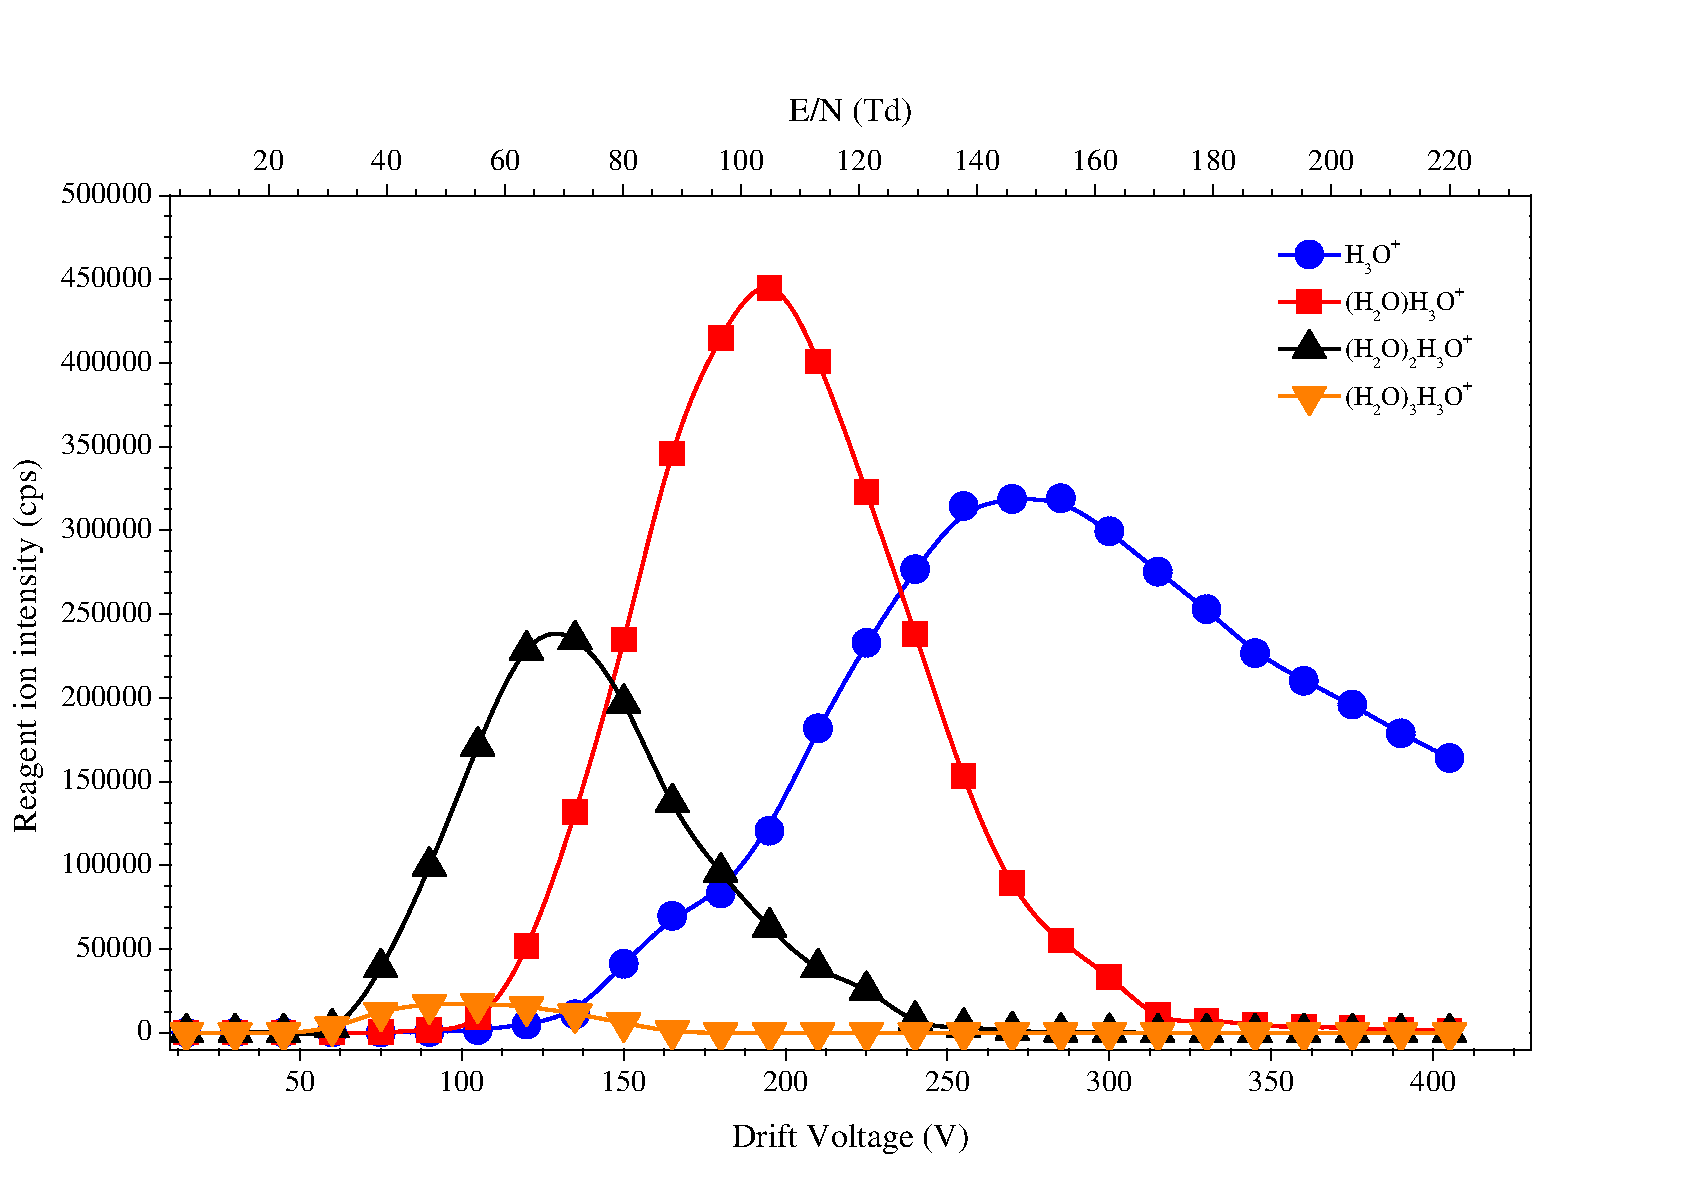
\includegraphics[width=0.8\linewidth]{pics/DPM_clusters_littoral.pdf}%water_DC.png}
\label{fig:ri1}}

\sidesubfloat[]{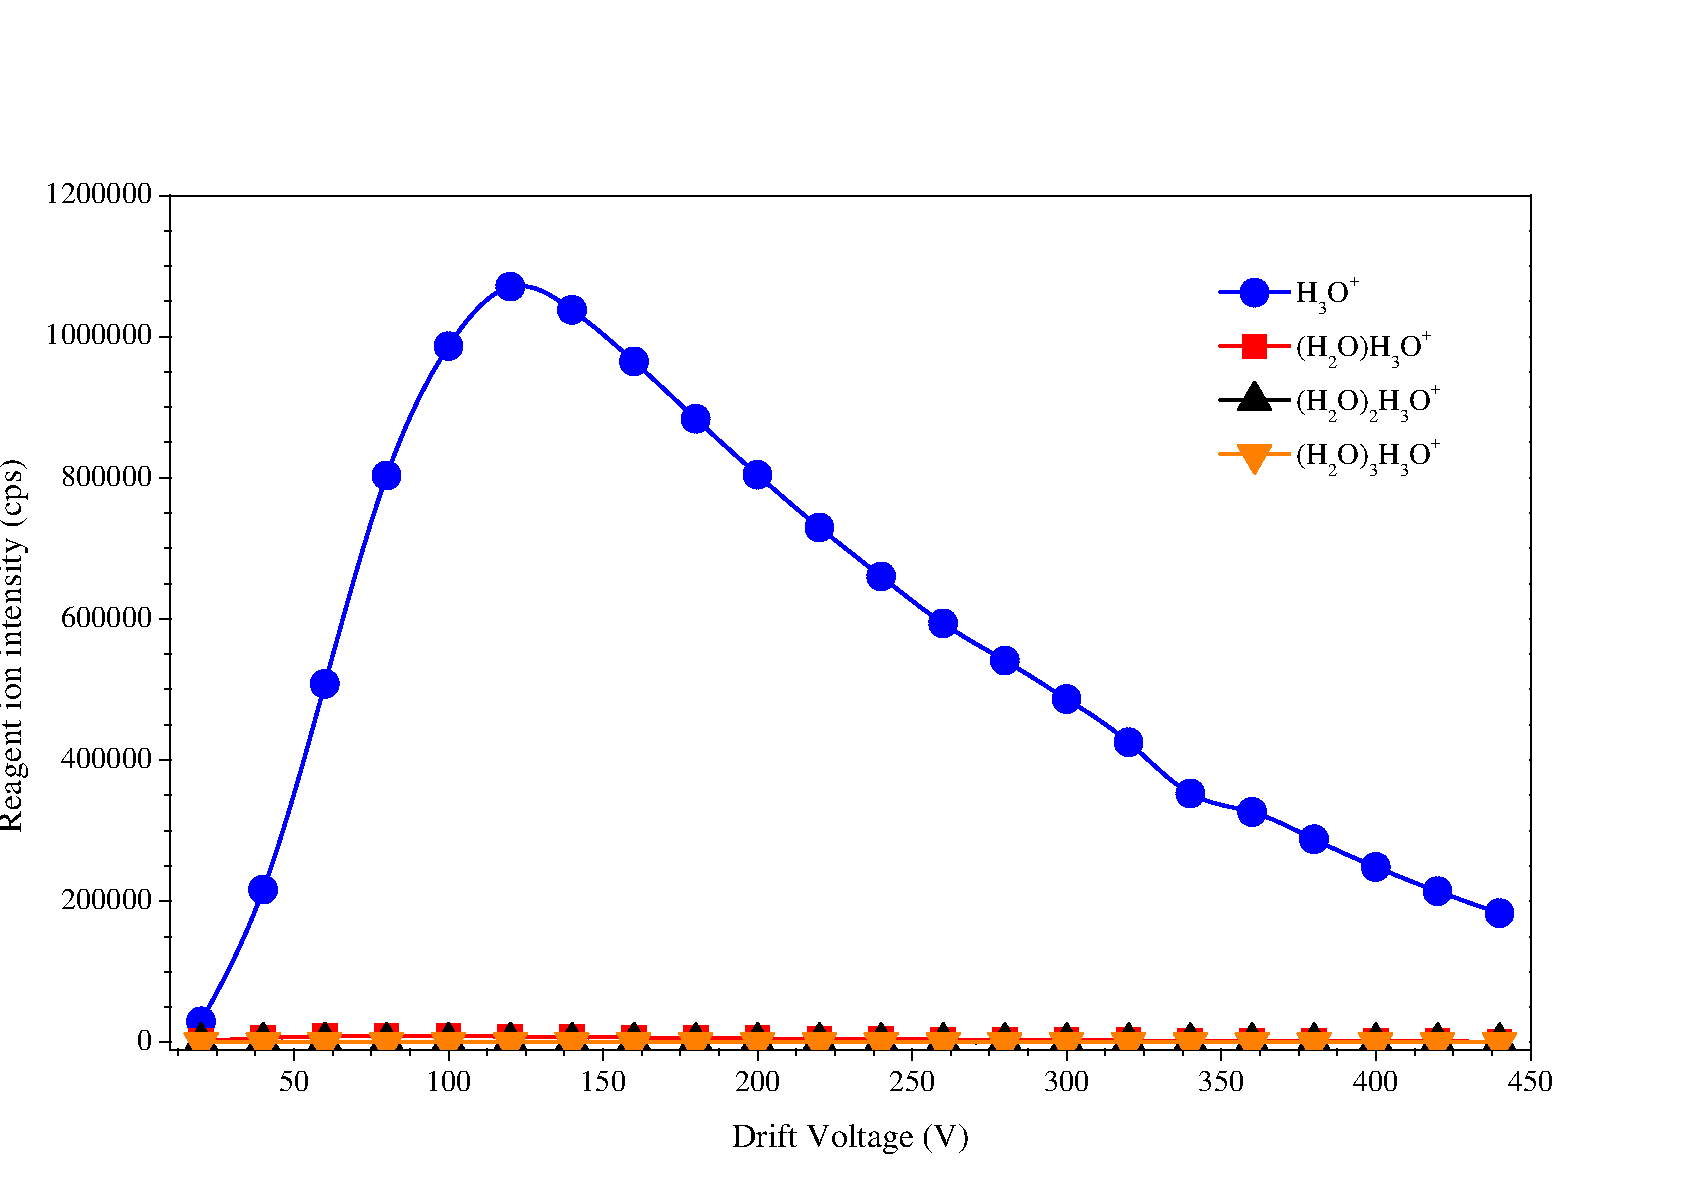
\includegraphics[width=0.8\linewidth]{pics/DPM_clusters_dry_RF.pdf}%water_RF.png}
\label{fig:ri2}}
\caption{Ion signal in counts per second (cps) for the reagent ions in (a) DC mode and (b) RF mode at 100$^{\circ}$C and 1 mbar. \textbf{Bottom one is from Lynx (MkII reactor)}}
\label{fig:ri}
\end{figure}




\section{Results and discussion}
\subsection{Measurement of illicit drugs in DC mode}

\subsubsection{Cocaine}



\begin{table}%[ht]
\centering
\caption{Proton affinity, PA, and Gibbs free energy, GB, of the main protonation sites of cocaine.}
\label{tb:co1}
\begin{tabular}{lcc}
\toprule
\textbf{Structure} &\textbf{PA (kJ/mol)} &\textbf{GB (kJ/mol)}\\ \toprule
Cocaine1H$^+$  & 1013 &   980    \\
Cocaine2H$^+$  &933 &   895    \\
\bottomrule
\end{tabular}
\end{table}

\begin{table}%[ht]
\centering
\caption[Energetics relative to cocaine and H$_3$O$^+$.]{Energetics relative to cocaine and H$_3$O$^+$ and, in brackets, to cocaine and (H$_2$O)H$_3$O$^+$. Note that m/z refers to the detected ion, i.e. where the charge remains, and that the neutral H$_2$O has been omitted in all the cases.}
\label{tb:co2}
\begin{tabular}{lccc}
\toprule
\textbf{Reaction or transition state}	&\textbf{m/z} &\textbf{$\Delta$H$_{298}$} &\textbf{$\Delta$G$_{298}$}\\
& &	\textbf{(kJ/mol)} &\textbf{(kJ/mol)} \\  \toprule
Cocaine1H$^+$  				&	304	& -328 (-170)  & -326 (-202)   \\ \midrule
(CocaineH$^+$ - MeOH) + MeOH   			&	272	& -138 (+20)	&-186 (-62)   \\ \midrule
(CocaineH - benzoic acid)$^+$ + benzoic acid &	182 & -272 (-114)  & -336 (-212)  \\ \midrule
(CocaineH - benzoyl) + benzoyl$^+$    	&	105	& -54 (+104)  & -104 (+20)  \\ \midrule
(Cocaine - benzoic acidH) + benzoic acidH$^+$& 123	& -88 (+70)  & -144  (-20) \\ \midrule
MeOH loss: TS2 for H migration O3 to O5& & -8 (+150)  & -9 (+115)  \\ \midrule
MeOH loss: TS2A for H migration O2 to O5& & -119 (+39)  & -111  (+13) \\ 
\bottomrule
\end{tabular}
\end{table}



\begin{figure}%[h]
\centering
\scalebox{0.5}{
\begin{tikzpicture}
\chemfig{[:180]**6(------)-[::210](=[::60]O^2)-[::-60]O^4>[::75](?[a])-[::30]-[::-60,1.4](<:[::60]H)(-[::-60]N^1?[b,{-}]-[::15])-[::90,1.1]-[::135,0.8]-[::45,1.1](?[b])(<[::0]H)-[::-60]?[a](<[::45](=[::60]O^3)-[::-60]O^5-[::60])}
%\chemfig{[:180]**6(------)-[::210](=[::60]O)-[::-60]O>[::75](?[a])-[::30]-[::-60,1.4](<:[::60]H)(-[::120]N?[b,{-}]-[::-15])-[::-30,1.1]-[::-90,0.8]-[::-90,1.1](?[b])(<[::105]H)-[::60]?[a](<[::45](=[::60]O)-[::-60]O-[::60])} %previous version with the N in opposite way
\end{tikzpicture}
}\label{fig:coc}
\caption{Cocaine}
\end{figure}

\begin{figure}
\begin{center}
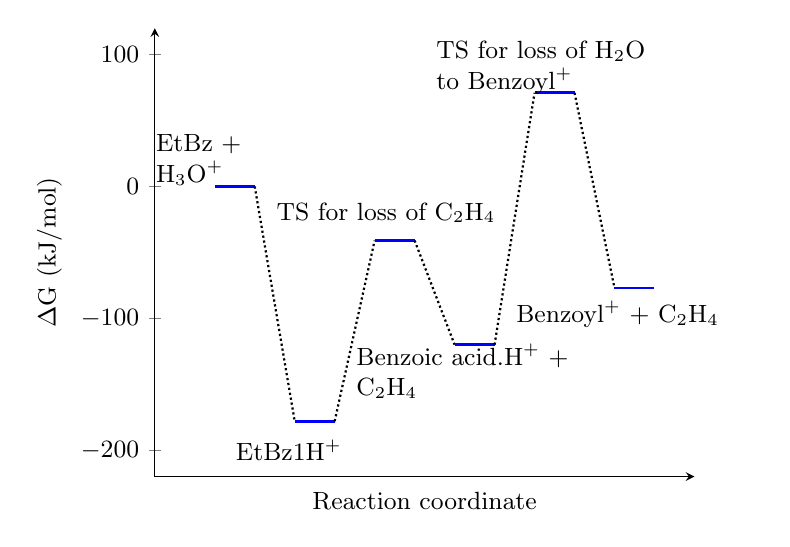
\begin{tikzpicture}[scale=1.0]
\tikzstyle{every node}=[font=\small]
\begin{axis}[clip=false,ylabel=$\Delta$G (kJ/mol),xlabel=Reaction coordinate,xtick=\empty,
legend pos=outer north east,xmin=0.5,xmax=14,ymax=120,ymin=-220,axis lines = left]
\addplot[color=black,draw=blue,line width=1pt] coordinates {(2,0)(3,0)};
\addplot[color=black,line width=0.8pt,densely dotted] coordinates {(3,0)(4,-178)};
\addplot[color=black,draw=blue,line width=1pt] coordinates {(4,-178)(5,-178)};
\addplot[color=black,line width=0.8pt,densely dotted] coordinates {(5,-178)(6,-41)};
\addplot[color=black,draw=blue,line width=1pt] coordinates {(6,-41)(7,-41)};
\addplot[color=black,line width=0.8pt,densely dotted] coordinates {(7,-41)(8,-120)};
\addplot[color=black,draw=blue,line width=1pt] coordinates {(8,-120)(9,-120)};
\addplot[color=black,line width=0.8pt,densely dotted] coordinates {(9,-120)(10,71)};
\addplot[color=black,draw=blue,line width=1pt] coordinates {(10,71)(11,71)};
\addplot[color=black,line width=0.8pt,densely dotted] coordinates {(11,71)(12,-77)};
\addplot[color=black,draw=blue,line width=1pt] coordinates {(12,-77)(13,-77)};
\node [text width=2cm] at (axis cs:2.5,20) {EtBz + H$_3$O$^+$};
\node [text width=2cm] at (axis cs:4.5,-200) {EtBz1H$^+$};
\node [text width=3cm] at (axis cs:6.5,-20) {TS for loss of C$_2$H$_4$};
\node [text width=3cm] at (axis cs:8.5,-140) {Benzoic acid.H$^+$ + C$_2$H$_4$};
\node [text width=3cm] at (axis cs:10.5,90) {TS for loss of H$_2$O to Benzoyl$^+$};
\node [text width=3cm] at (axis cs:12.5,-97) {Benzoyl$^+$ + C$_2$H$_4$};
%\node at (2.5,3) {\includegraphics[scale=0.1]{rea1.pdf}};
%\node at (axis cs:2.1,-10) {\includegraphics[scale=0.06,angle=90]{r1.pdf}};
%\node at (axis cs:3.2,-10) {\includegraphics[scale=0.06,angle=90]{r2.pdf}};
%\node at (axis cs:4.3,50) {\includegraphics[scale=0.08,angle=90]{t1.pdf}};
%\node at (axis cs:6.9,-35) {\includegraphics[scale=0.08,angle=90]{p1.pdf}};
\end{axis}
\end{tikzpicture}
\end{center}
\caption{$\Delta$G for reaction of H$_3$O$^+$ with EtBz –- Example of the data from Peter Watts}\label{fig:trans.example}
\end{figure}

\newpage

\begin{table}%[ht]
\centering
\caption[Energetics relative to ethyl benzoate and H$_3$O$^+$.]{Energetics relative to ethyl benzoate and H$_3$O$^+$. Note that m/z refers to the detected ion, i.e. where the charge remains, and that the neutral H$_2$O has been omitted in all the cases.}
\label{tb:eb2}
\begin{tabular}{lccc}
\toprule
\textbf{Reaction or transition state}	&\textbf{m/z} &\textbf{$\Delta$H$_{298}$} &\textbf{$\Delta$G$_{298}$}\\
& &	\textbf{(kJ/mol)} &\textbf{(kJ/mol)} \\  \toprule
EtBz1H$^+$   					&	151	& -180  & -178   \\ \midrule
EtBz2H$^+$   					&	151	& -95  & -97   \\ \midrule
Benzoyl$^+$  + EtOH				&	105	& -36  & -83   \\ \midrule
TS to above, i.e. to 2H$^+$		&		& -3  & +2   \\ \midrule
Benzoic acid.H$^+$ + C$_2$H$_4$	&	123	& -74  & -120   \\ \midrule
TS1 for loss of ethene from 1H$^+$	&		& -36  & -41   \\ \midrule
TS2 for loss of ethene from 2H$^+$	&		& -15  & -14   \\ \midrule
Benzoyl$^+$  + C$_2$H$_4$ + H$_2$O	&	105	& +15  & -77   \\ \midrule
%\multicolumn{2}{l}{TS3 to above(loss of H$_2$O from benzoic acid.H$^+$)}		& +98  & +52   \\ \midrule
TS3 to above, i.e.	&		&   &    \\ 
loss of H$_2$O from benzoic acid.H$^+$	&		& +98  & +52   \\ \midrule
Benzene.H$^+$	+ C$_2$H$_4$ + H$_2$O &	79	& +34  & -132   \\ 
\bottomrule
\end{tabular}
\end{table}


\begin{figure}%[h]
\begin{center}
\schemedebug{false}
\schemestart[0,1,thick]
\chemname{\scalebox{0.4}{\chemfig{**6(----(-[::-60](=[::60]O^1)-[::-60]O^2(-[::60]-[::-60]))--)}
}\+\chemfig{H_3O^+}}{Ethyl benzoate}
\arrow(nph.south--aa7)[-150,2]
		\chemname{\scalebox{0.4}{\chemfig{**6(----(-[::-60](-[,0.2,,,draw=none]\+)(-[::60]O-[::-60]H)-[::-60]O(-[::60]-[::-60]))--)}
}}{Ethyl benzoate 1H$^+$}
	\arrow[-90]
		\chemname{\scalebox{0.4}{\chemfig{**6(----(-[::-60](-[,0.2,,,draw=none]\+)(-[::60]O-[::-60]H)-[::-60]O(-[@{db}::-30]-[@{a1}::90]-[@{db2}::90]H-[@{a2}::90,,,,draw=none]))--)}
    	\chemmove{\draw(db)..controls +(120:4mm) and +(150:4mm)..(a1);
    	\draw(db2)..controls +(-60:4mm) and +(-30:4mm)..(a2);}}%\+\chemfig{H_2O}
                }{TS1 from 1H$^+$}
	\arrow(aa11--ba)[-90]
    	\chemname{\scalebox{0.4}{\chemfig{**6(----(-[::-60](-[,0.2,,,draw=none]\+)(-[::60]O-[::-60]H)-[::-60]O(-[::60]H))--)}
}}{Benzoic acid.H$^+$}
	\arrow(@ba--)[-90]
    	\chemname{\scalebox{0.4}{\chemfig{**6(----(-[::-60](-[,0.2,,,draw=none]\+)(-[@{a3}::60]O-[@{db3}::-60]H-[@{a4}::-120,1.5,,,draw=none])-[@{db4}::-60]O(-[::60]H))--)}
        \chemmove{\draw(db3)..controls +(0:4mm) and +(90:4mm)..(a3);
    	\draw(db4)..controls +(270:4mm) and +(270:4mm)..(a4);}
        }}{TS3 (loss of water)}
	\arrow(aa10--aa2)[0,3.7]
    	\chemname{\scalebox{0.4}{\chemfig{**6(----(-[::-60](-[,0.2,,,draw=none]\+)=[::60]O)--)}}}{Benzoyl$^+$}
\arrow(@nph.south--aa3)[-30,2]
		\chemname{\scalebox{0.4}{\chemfig{**6(----(-[::-60](=[::60]O)-[::-60]O^+(-[::-60]H)(-[::60]-[::-60]))--)}
}}{Ethyl benzoate 2H$^+$}
	\arrow(.south--aa4)[-135,2.5]
    	\chemname{\scalebox{0.4}{\chemfig{**6(----(-[::-60](*6(-O^+(-[::-60]H)-[@{db6}]-[@{a6}]-H-[@{a5},,,,draw=none]O=[@{db5}])))--)}
		\chemmove{\draw(db5)..controls +(60:4mm) and +(0:4mm)..(a5);
    	\draw(db6)..controls +(180:4mm) and +(240:4mm)..(a6);}
		}}{TS2 from 2H$^+$}
     \arrow(@aa3.south--@aa2)
    \arrow(@aa4.mid west--@ba)
    \arrow(@aa7--aa8.)[0,1.3]
        	\chemname{\scalebox{0.4}{\chemfig{**6(----(-[::-60](*6(-O^+(-[@{db6}::-60,,,,draw=none])-(-[::-60])-[,,,,draw=none]-[,,,,draw=none]H(-[@{a6}::-240,,,,draw=none])-[@{a5}]O-[@{db5}])))--)}
		\chemmove{\draw(a5)..controls +(0:4mm) and +(60:4mm)..(db5);
		\draw(db6)..controls +(-120:10mm) and +(-90:10mm)..(a6);}
		}}{TS from 1H$^+$ to 2H$^+$}
		\arrow(.east--aa3)[0,1.3]
\schemestop
\end{center}
\caption{Ethyl benzoate}\label{fig:eb1}
\end{figure}





\subsubsection{Ecstasy}

\begin{figure}%[h]
\centering
\scalebox{0.5}{
\chemfig{*6(=-*5(-O--O-?[a]=)--=(--[::60](-[::60])-[::-60]N(-[::-60]H)-[::60])-)}}
\caption{MDMA}\label{fig:mdma}
\end{figure}



\subsubsection{Codeine}

\begin{figure}%[h]
\centering
\scalebox{0.5}{
\chemfig{[:-120]**6(-(-O@{a1}-[::300])-?[a]-*6(-(<[::130,1]-[::-45,1.5,,,line width=3pt]?[b])*6(-(<:[::-80,1.25]O?[a])(<[::0]H)-(<:O-[::60]H)-=-)-(<[::-30]H)-(<:[::-105]H)(-N?[b,{>}]-[::-30])--)---)}}
\caption{codeine}\label{fig:cod}
\end{figure}



\subsubsection{Morphine}


\begin{figure}%[h]
\centering
\scalebox{0.5}{
\begin{tikzpicture}\chemfig{[:-120]**6(-(-O-[::-60]H)-?[a]-*6(-(<[::130,1]-[::-45,1.5,,,line width=3pt]?[b])*6(-(<:[::-80,1.25]O?[a])(<[::0]H)-(<:O-[::60]H)-=-)-(<[::-30]H)-(<:[::-105]H)(-N?[b,{>}]-[::-30])--)---)}
\end{tikzpicture}}
\caption{morphine}\label{fig:mor}
\end{figure}



\subsubsection{Heroin}

\begin{figure}%[h]
\centering
\scalebox{0.5}{
\begin{tikzpicture}
\chemfig{[:-120]**6(-(-O@{a1}-[::300](=[@{db}::-60]O)-[::60])-?[a]-*6(-(<[::130,1]-[::-45,1.5,,,line width=3pt]?[b])*6(-(<:[::-80,1.25]O?[a])(<[::0]H)-(<:\chemabove{O}{\scriptstyle\oplus}-[::60](-[::-60])=[::60]O)-=-)-(<[::-30]H)-(<:[::-105]H)(-N?[b,{>}]-[::-30])--)---)}
\end{tikzpicture}}
\caption{Heroin}\label{fig:her}
\end{figure}


\subsubsection{Cocaine-related compounds}

\begin{figure}%[h]
\begin{center}
\begin{subfloatrow}
\sidesubfloat[]{\scalebox{0.5}{
\chemfig{**6(------)-[::210](=[::60]O)-[::-60]O(-[::60]H-[::-60,,,,white])}}\label{fig:ba}}
\quad\quad
\sidesubfloat[]{\scalebox{0.5}{
\chemfig{**6(------)-[::210](=[::60]O)-[::-60]O(-[::60]-[::-60,,,,white])}}\label{fig:mb2}}
\quad\quad
\sidesubfloat[]{\scalebox{0.5}{
\chemfig{**6(------)-[::210](=[::60]O)-[::-60]O(-[::60]-[::-60])}}\label{fig:eb}}
\end{subfloatrow}
\bigskip
%\begin{subfloatrow}
\sidesubfloat[]{\scalebox{0.5}{
\chemfig{**6(------)-[::210](=[::60]O)-[::-60]O(-[::60](-[::60])-[::-60])}}\label{fig:ib}}
\quad\quad
\sidesubfloat[]{\scalebox{0.5}{
\chemfig{**6(------)-[::210](=[::60]O)-[::-60]O-[::60](=[::60]O)-[::-60]**6(------)}}\label{fig:ban}}
%\end{subfloatrow}
\end{center}
\caption{Structure of (a) benzoic acid,  (b) methyl benzoate, (c) ethyl benzoate, (d) isopropyl benzoate and (e) benzoic anhydride.}\label{fig:cocr}
\end{figure}




\begin{table}%[ht]
\centering
\caption{Proton affinity, PA, and Gibbs free energy, GB, of the main protonation sites of methyl benzoate.}
\label{tb:mb1}
\begin{tabular}{lcc}
\toprule
\textbf{Structure} &\textbf{PA (kJ/mol)} &\textbf{GB (kJ/mol)}\\ \toprule
MeBz1H$^+$  & 839 &   808    \\
MeBz2H$^+$  & 764 &   741    \\
\bottomrule
\end{tabular}
\end{table}

\begin{table}%[ht]
\centering
\caption[Energetics relative to methyl benzoate and H$_3$O$^+$.]{Energetics relative to methyl benzoate and H$_3$O$^+$. Note that m/z refers to the detected ion, i.e. where the charge remains, and that the neutral H$_2$O has been omitted in all the cases.}
\label{tb:mb2}
\begin{tabular}{lccc}
\toprule
\textbf{Reaction or transition state}	&\textbf{m/z} &\textbf{$\Delta$H$_{298}$} &\textbf{$\Delta$G$_{298}$}\\
& &	\textbf{(kJ/mol)} &\textbf{(kJ/mol)} \\  \toprule
MeBz1H$^+$   					&	137	& -155  & -155   \\ \midrule
Benzoyl$^+$ + MeOH				&	105	& -29  & -82   \\ \midrule
TS to above, i.e. to 2H$^+$\footnote[2]{I don't get this}&		& +15  	& +14\\ \midrule
MeBz2H$^+$ 						&	137	& -80  & -88   \\ 
\bottomrule
\end{tabular}
\end{table}

\begin{figure}%[h]
\begin{center}
\scalebox{0.5}{
\chemfig{**6(----(-[::-60](=[::60]O^1)-[::-60]O^2(-[::60]))--)}
}
\end{center}
\caption{Methyl benzoate}
\end{figure}


\begin{figure}%[h]
\centering
\scalebox{0.5}{
\begin{tikzpicture}
\chemfig{[:180]**6(------)-[::210](=[::60]O^2)-[::-60]O^4>[::75](?[a])-[::30]-[::-60,1.4](<:[::60]H)(-[::-60]N^1?[b,{-}]-[::15])-[::90,1.1]-[::135,0.8]-[::45,1.1](?[b])(<[::0]H)-[::-60]?[a](<[::45](=[::60]O^3)-[::-60]O^5-[::60]H)}
\end{tikzpicture}}
\caption{Benzoyl ecgonine}\label{fig:be}
\end{figure}


\begin{figure}%[h]
\centering
\scalebox{0.5}{
\begin{tikzpicture}
\chemfig{[:180]**6(------)-[::210](=[::60]O^2)-[::-60]O^4>[::75](?[a])-[::30]-[::-60,1.4](<:[::60]H)(-[::-60]N^1?[b,{-}]-[::15])-[::90,1.1]-[::135,0.8]-[::45,1.1](?[b])(<[::0]H)-[::-60]?[a](<[::45](=[::60]O^3)-[::-60]O^5-[::60]-[::-60])}
%\chemfig{[:180]**6(------)-[::210](=[::60]O)-[::-60]O>[::75](?[a])-[::30]-[::-60,1.4](<:[::60]H)(-[::120]N?[b,{-}]-[::-15])-[::-30,1.1]-[::-90,0.8]-[::-90,1.1](?[b])(<[::105]H)-[::60]?[a](<[::45](=[::60]O)-[::-60]O-[::60])} %previous version with the N in opposite way
\end{tikzpicture}
}\label{fig:cocet}
\caption{Cocaethylene}
\end{figure}




\begin{table}%[ht]
\centering
\caption{Proton affinity, PA, and Gibbs free energy, GB, of the main protonation sites of methyl ecgonine.}
\label{tb:me1}
\begin{tabular}{lcc}
\toprule
\textbf{Structure} &\textbf{PA (kJ/mol)} &\textbf{GB (kJ/mol)}\\ \toprule
MeEcg1H$^+$  & 996 &   965    \\
MeEcg3H$^+$  & 906 &   873    \\
\bottomrule
\end{tabular}
\end{table}

\begin{table}%[ht]
\centering
\caption[Energetics relative to methyl ecgonine and H$_3$O$^+$.]{Energetics relative to methyl ecgonine and H$_3$O$^+$. Note that m/z refers to the detected ion, i.e. where the charge remains, and that the neutral H$_2$O has been omitted in all the cases.}
\label{tb:me2}
\begin{tabular}{lccc}
\toprule
\textbf{Reaction or transition state}	&\textbf{m/z} &\textbf{$\Delta$H$_{298}$} &\textbf{$\Delta$G$_{298}$}\\
& &	\textbf{(kJ/mol)} &\textbf{(kJ/mol)} \\  \toprule
MeEcg1H$^+$   				&	200	& -312  & -312   \\ \midrule
(MeEcgH - MeOH)$^+$ + MeOH	&	168	& -118  & -171   \\ \midrule
TS for loss of MeOH			&		& +4  	& 0   		\\ \midrule
(MeEcgH - H$_2$O)$^+$ + H$_2$O	&	182	& -260  & -320   \\ 
\bottomrule
\end{tabular}
\end{table}

\begin{figure}%[h]
\centering
\scalebox{0.5}{
\begin{tikzpicture}
\chemfig{[:-30]O^4(-[::180]H)>[::60](?[a])-[::45]-[::-60,1.4](<:[::60]H)(-[::-60]N^1?[b,{-}]-[::15])-[::90,1.1]-[::135,0.8]-[::45,1.1](?[b])(<[::0]H)-[::-60]?[a](<[::45](=[::60]O^3)-[::-60]O^5-[::60])}
\end{tikzpicture}}
\caption{Methyl ecgonine}\label{fig:me}
\end{figure}



\begin{figure}%[h]
\centering
\scalebox{0.5}{
\begin{tikzpicture}
\chemfig{[:30](?[a])-[::45]-[::-60,1.4](<:[::60]H)(-[::-60]N?[b,{-}]-[::15])-[::90,1.1]-[::135,0.8]-[::45,1.1](?[b])(<[::0]H)-[::-60]?[a,{=}](<[::45](=[::60]O)-[::-60]O-[::60])}
\end{tikzpicture}}
\caption{Methyl ecgonidine}\label{fig:med}
\end{figure}



\begin{figure}%[h]
\centering
\vspace{1cm}
\sidesubfloat[]{\scalebox{0.6}{\chemfig{[:30]-[::-60]-[::60]O-[::-60]-[::60]-[::-60]O-[::60]-[::-60]-[::60]O-[::-60]-[::60]}}}\label{fig:dgde1}
\quad
\sidesubfloat[]{\scalebox{0.6}{\chemfig{[:30]-[::-60]O-[::60]-[::-60]-[::60]O-[::-60]-[::60]-[::-60]O-[::60]}}}\label{fig:dgde2}
\vspace{1cm}
\caption{Structure of (a) diethylene glycol diethyl ether and (b) diethylene glycol dimethyl ether}\label{fig:dgde}
\end{figure}

























\subsection{Measurement of illicit drugs in RF mode}


\subsection{Nitroanilines}

\begin{figure}
\vspace{0.5cm}
  \sidesubfloat[]{\scalebox{0.7}{\begin{tikzpicture}\chemfig{**6(---(-[::-60]N(-[::60]H)-[::-60]H)-(-[::-60]N^{+}(=[::60]O)-[::-60]O^{-})--)}\end{tikzpicture}}\label{fig:nit1}}
\qquad
  \sidesubfloat[]{\scalebox{0.7}{\begin{tikzpicture}\chemfig{
**6(--(-[::-60]N(-[::60]H)-[::-60]H)--(-[::-60]N^{+}(=[::60]O)-[::-60]O^{-})--)}\end{tikzpicture}}\label{fig:nit2}}
\qquad
  \sidesubfloat[]{\scalebox{0.7}{\begin{tikzpicture}\chemfig{
**6(-(-[::-60]N(-[::60]H)-[::-60]H)---(-[::-60]N^{+}(=[::60]O)-[::-60]O^{-})--)}\end{tikzpicture}}\label{fig:nit3}}
  \caption{Structure of (a) 2-nitroaniline, (b) 3-nitroaniline and (c) 4-nitroaniline.}\label{fig:nit}
\end{figure}


\begin{figure}%[h]
\centering
\sidesubfloat[]{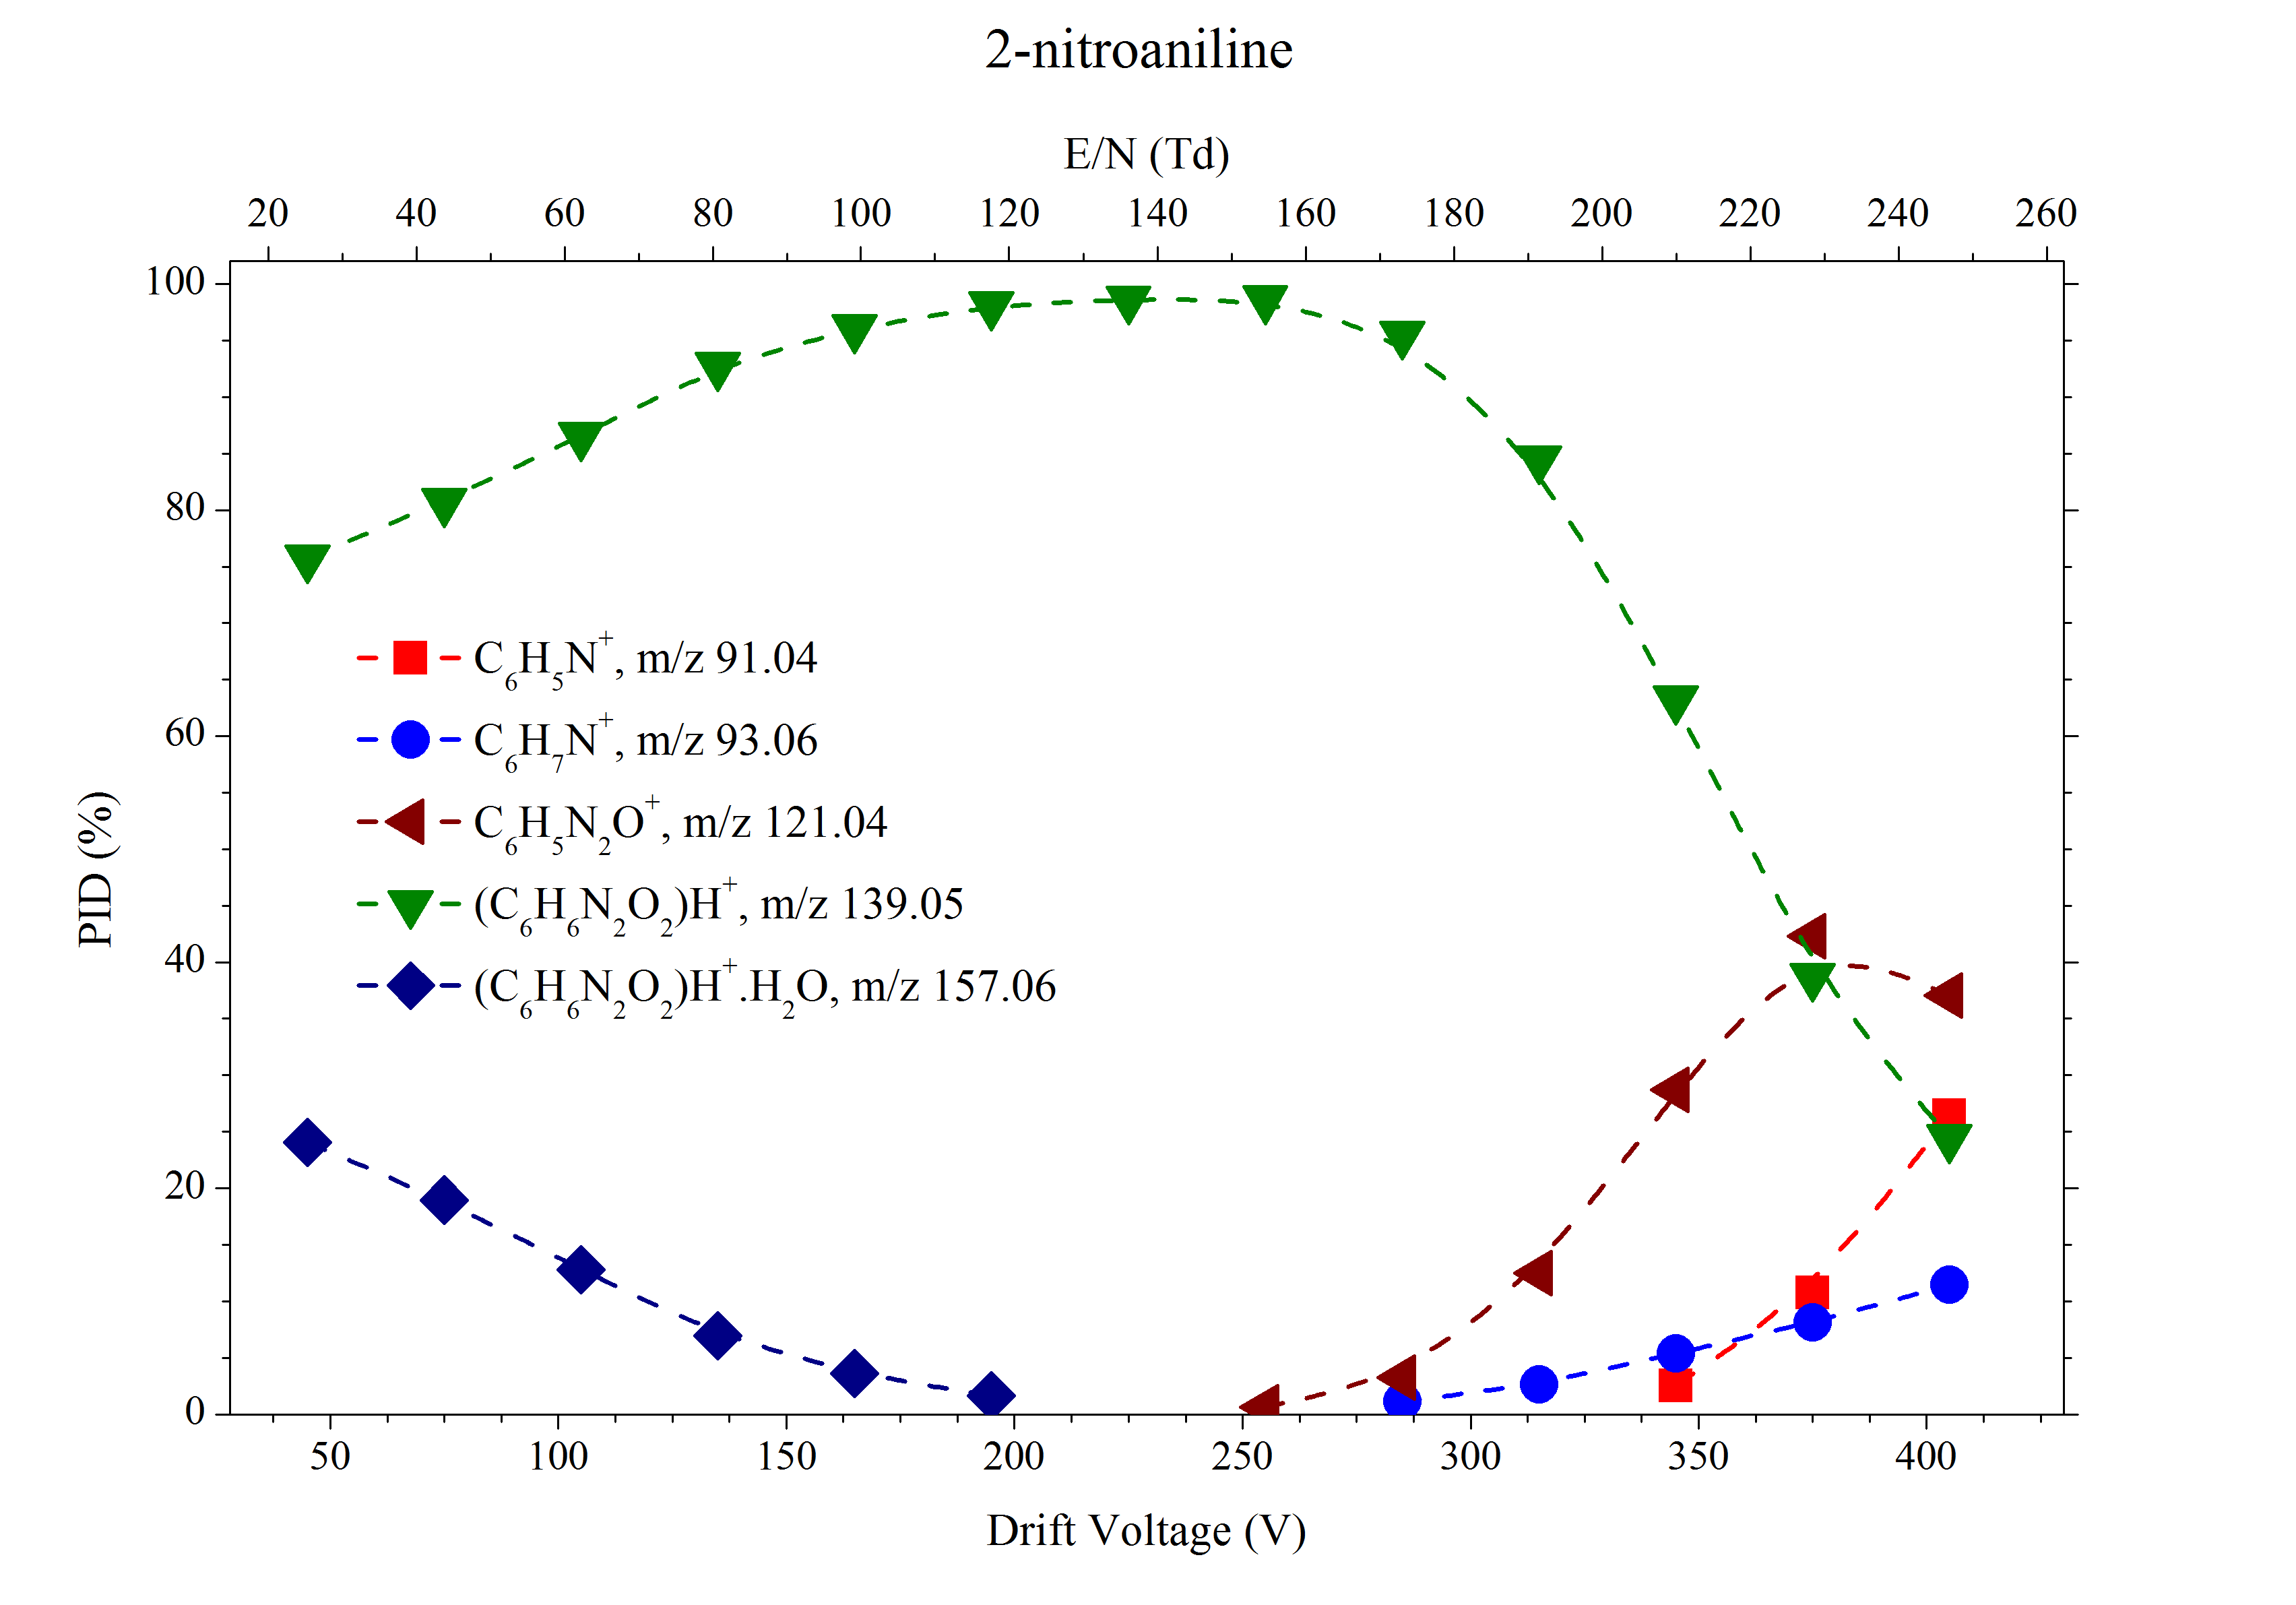
\includegraphics[width=0.6\linewidth]{pics/2-NA-h3o_DC.png}}

\sidesubfloat[]{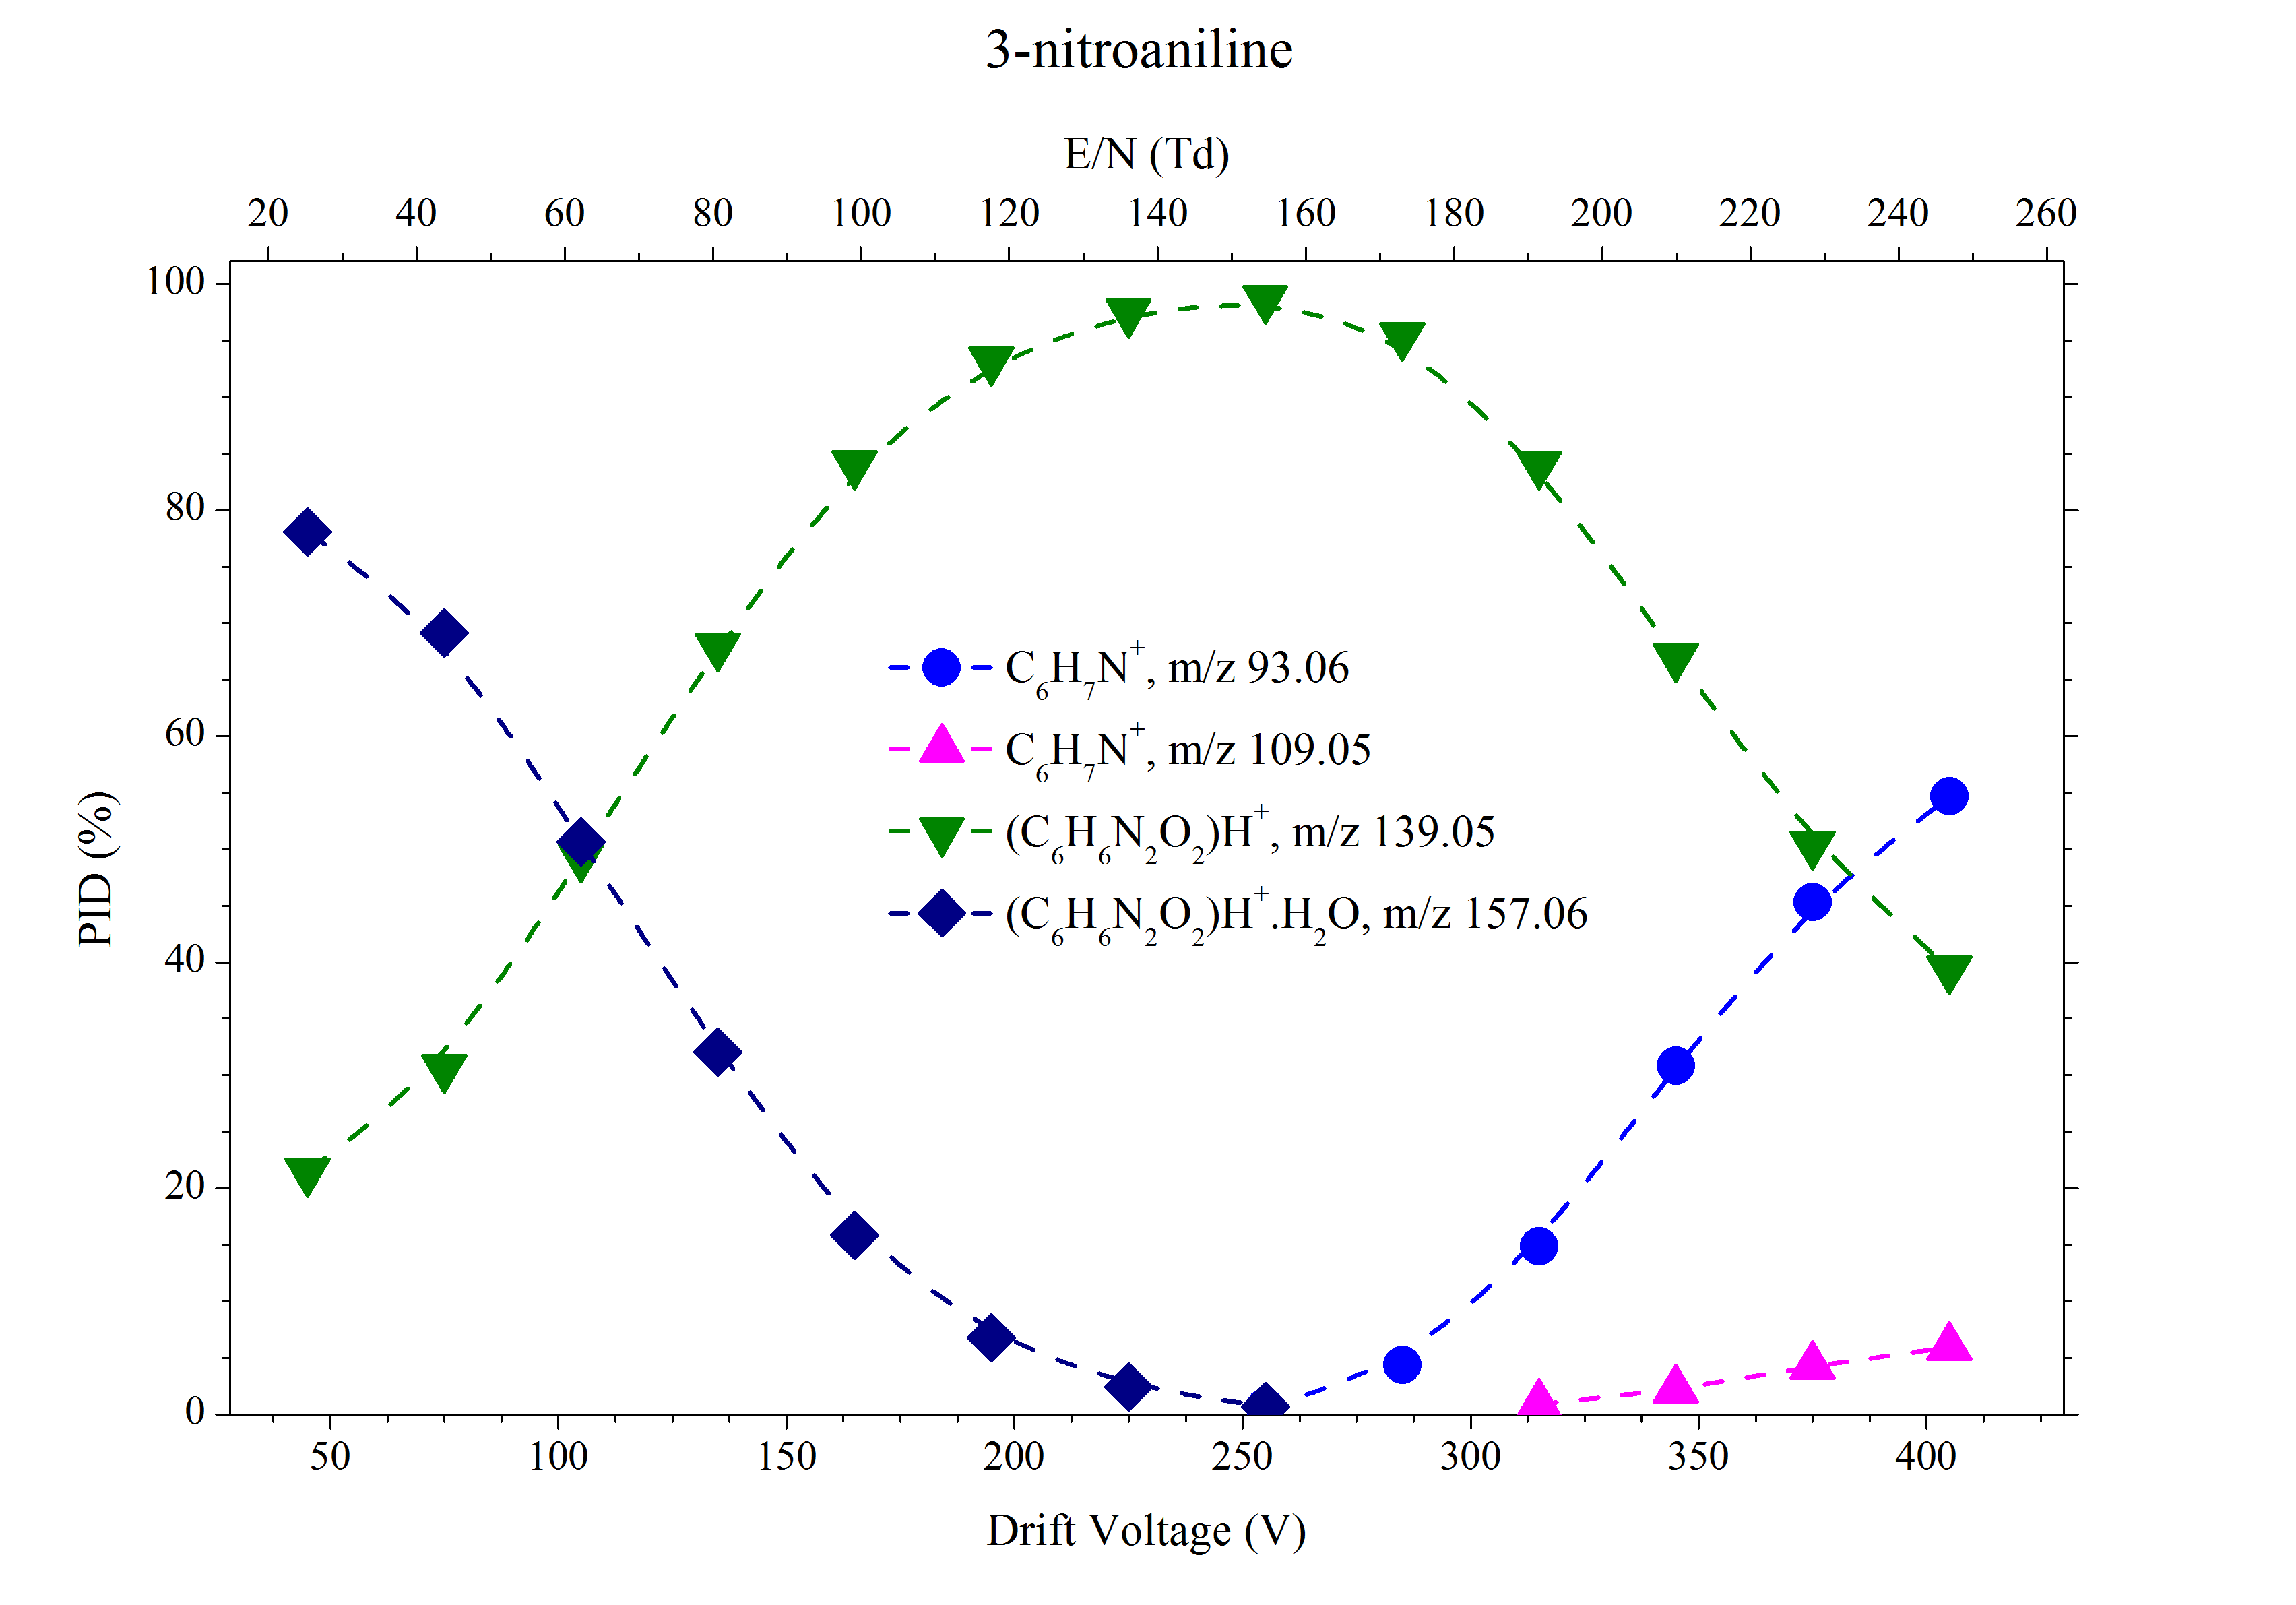
\includegraphics[width=0.6\linewidth]{pics/3-NA-h3o_DC.png}}

\sidesubfloat[]{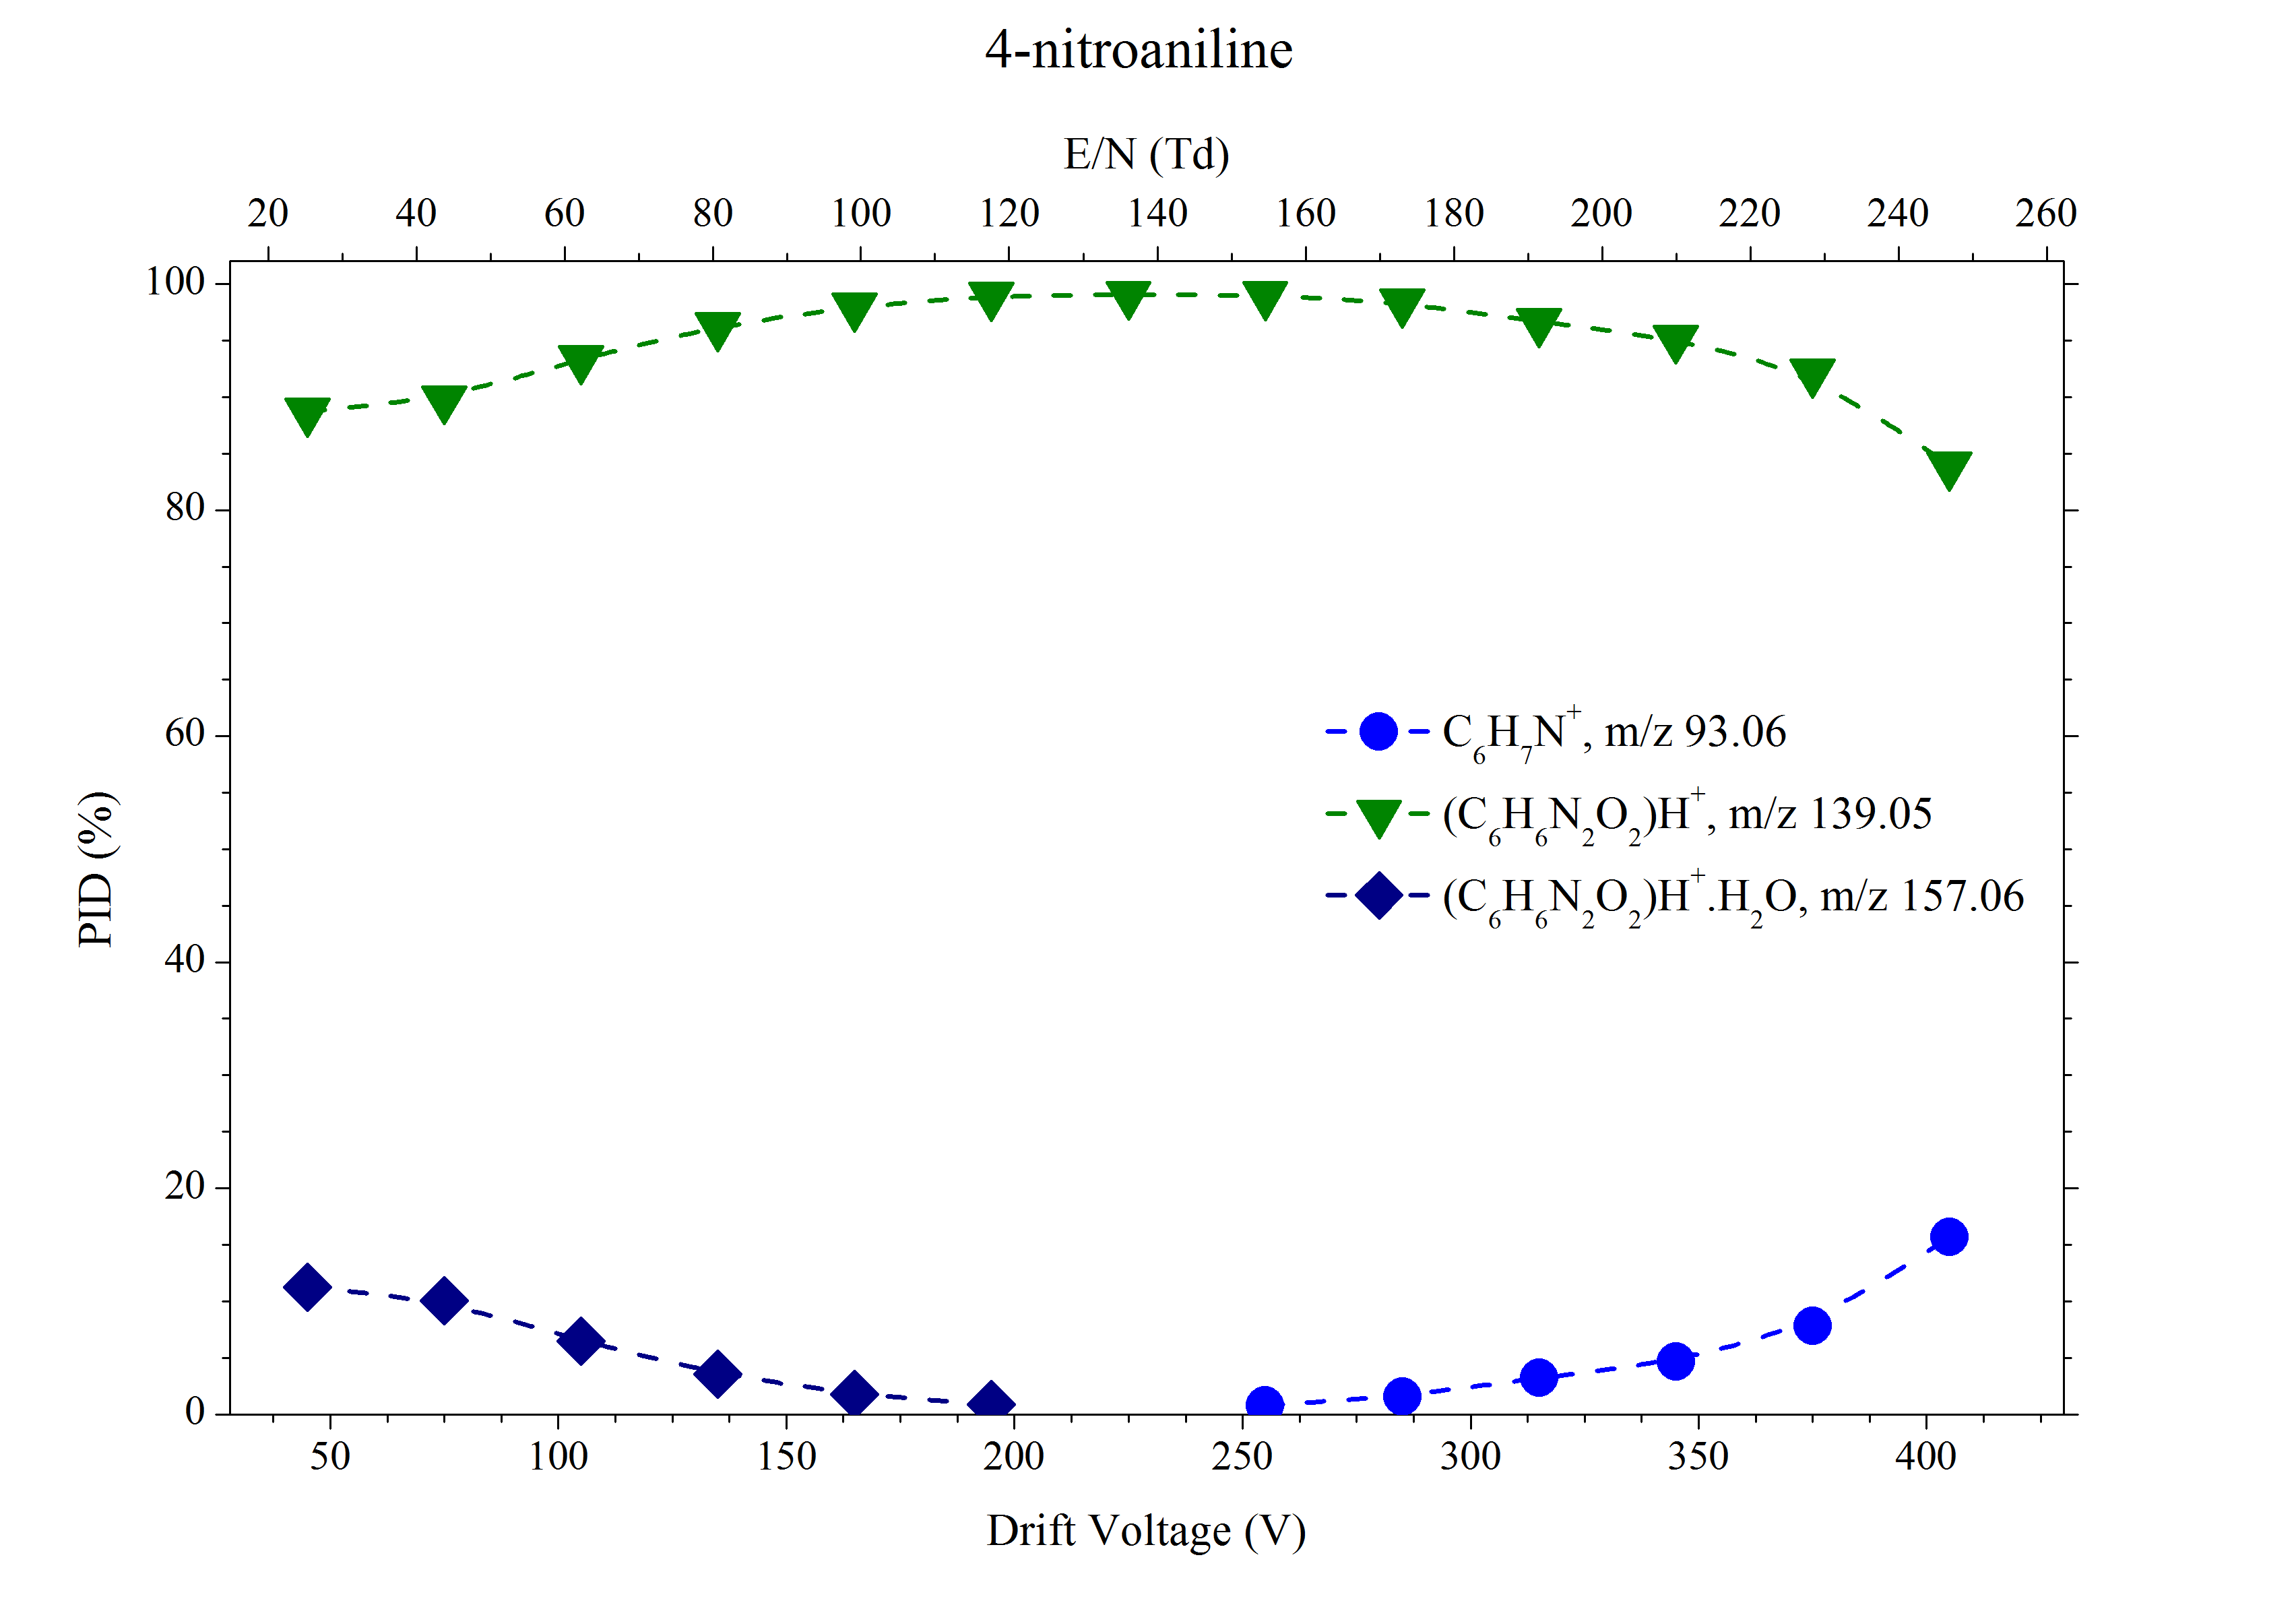
\includegraphics[width=0.6\linewidth]{pics/4-NA-h3o_DC.png}}
\caption{PID plots of (a) 2-nitroaniline, (b) 3-nitroaniline and (c) 4-nitroaniline, H3O+, DC mode}
\label{fig:na_h3o_dc}
\end{figure}

\begin{figure}%[h]
\centering
\sidesubfloat[]{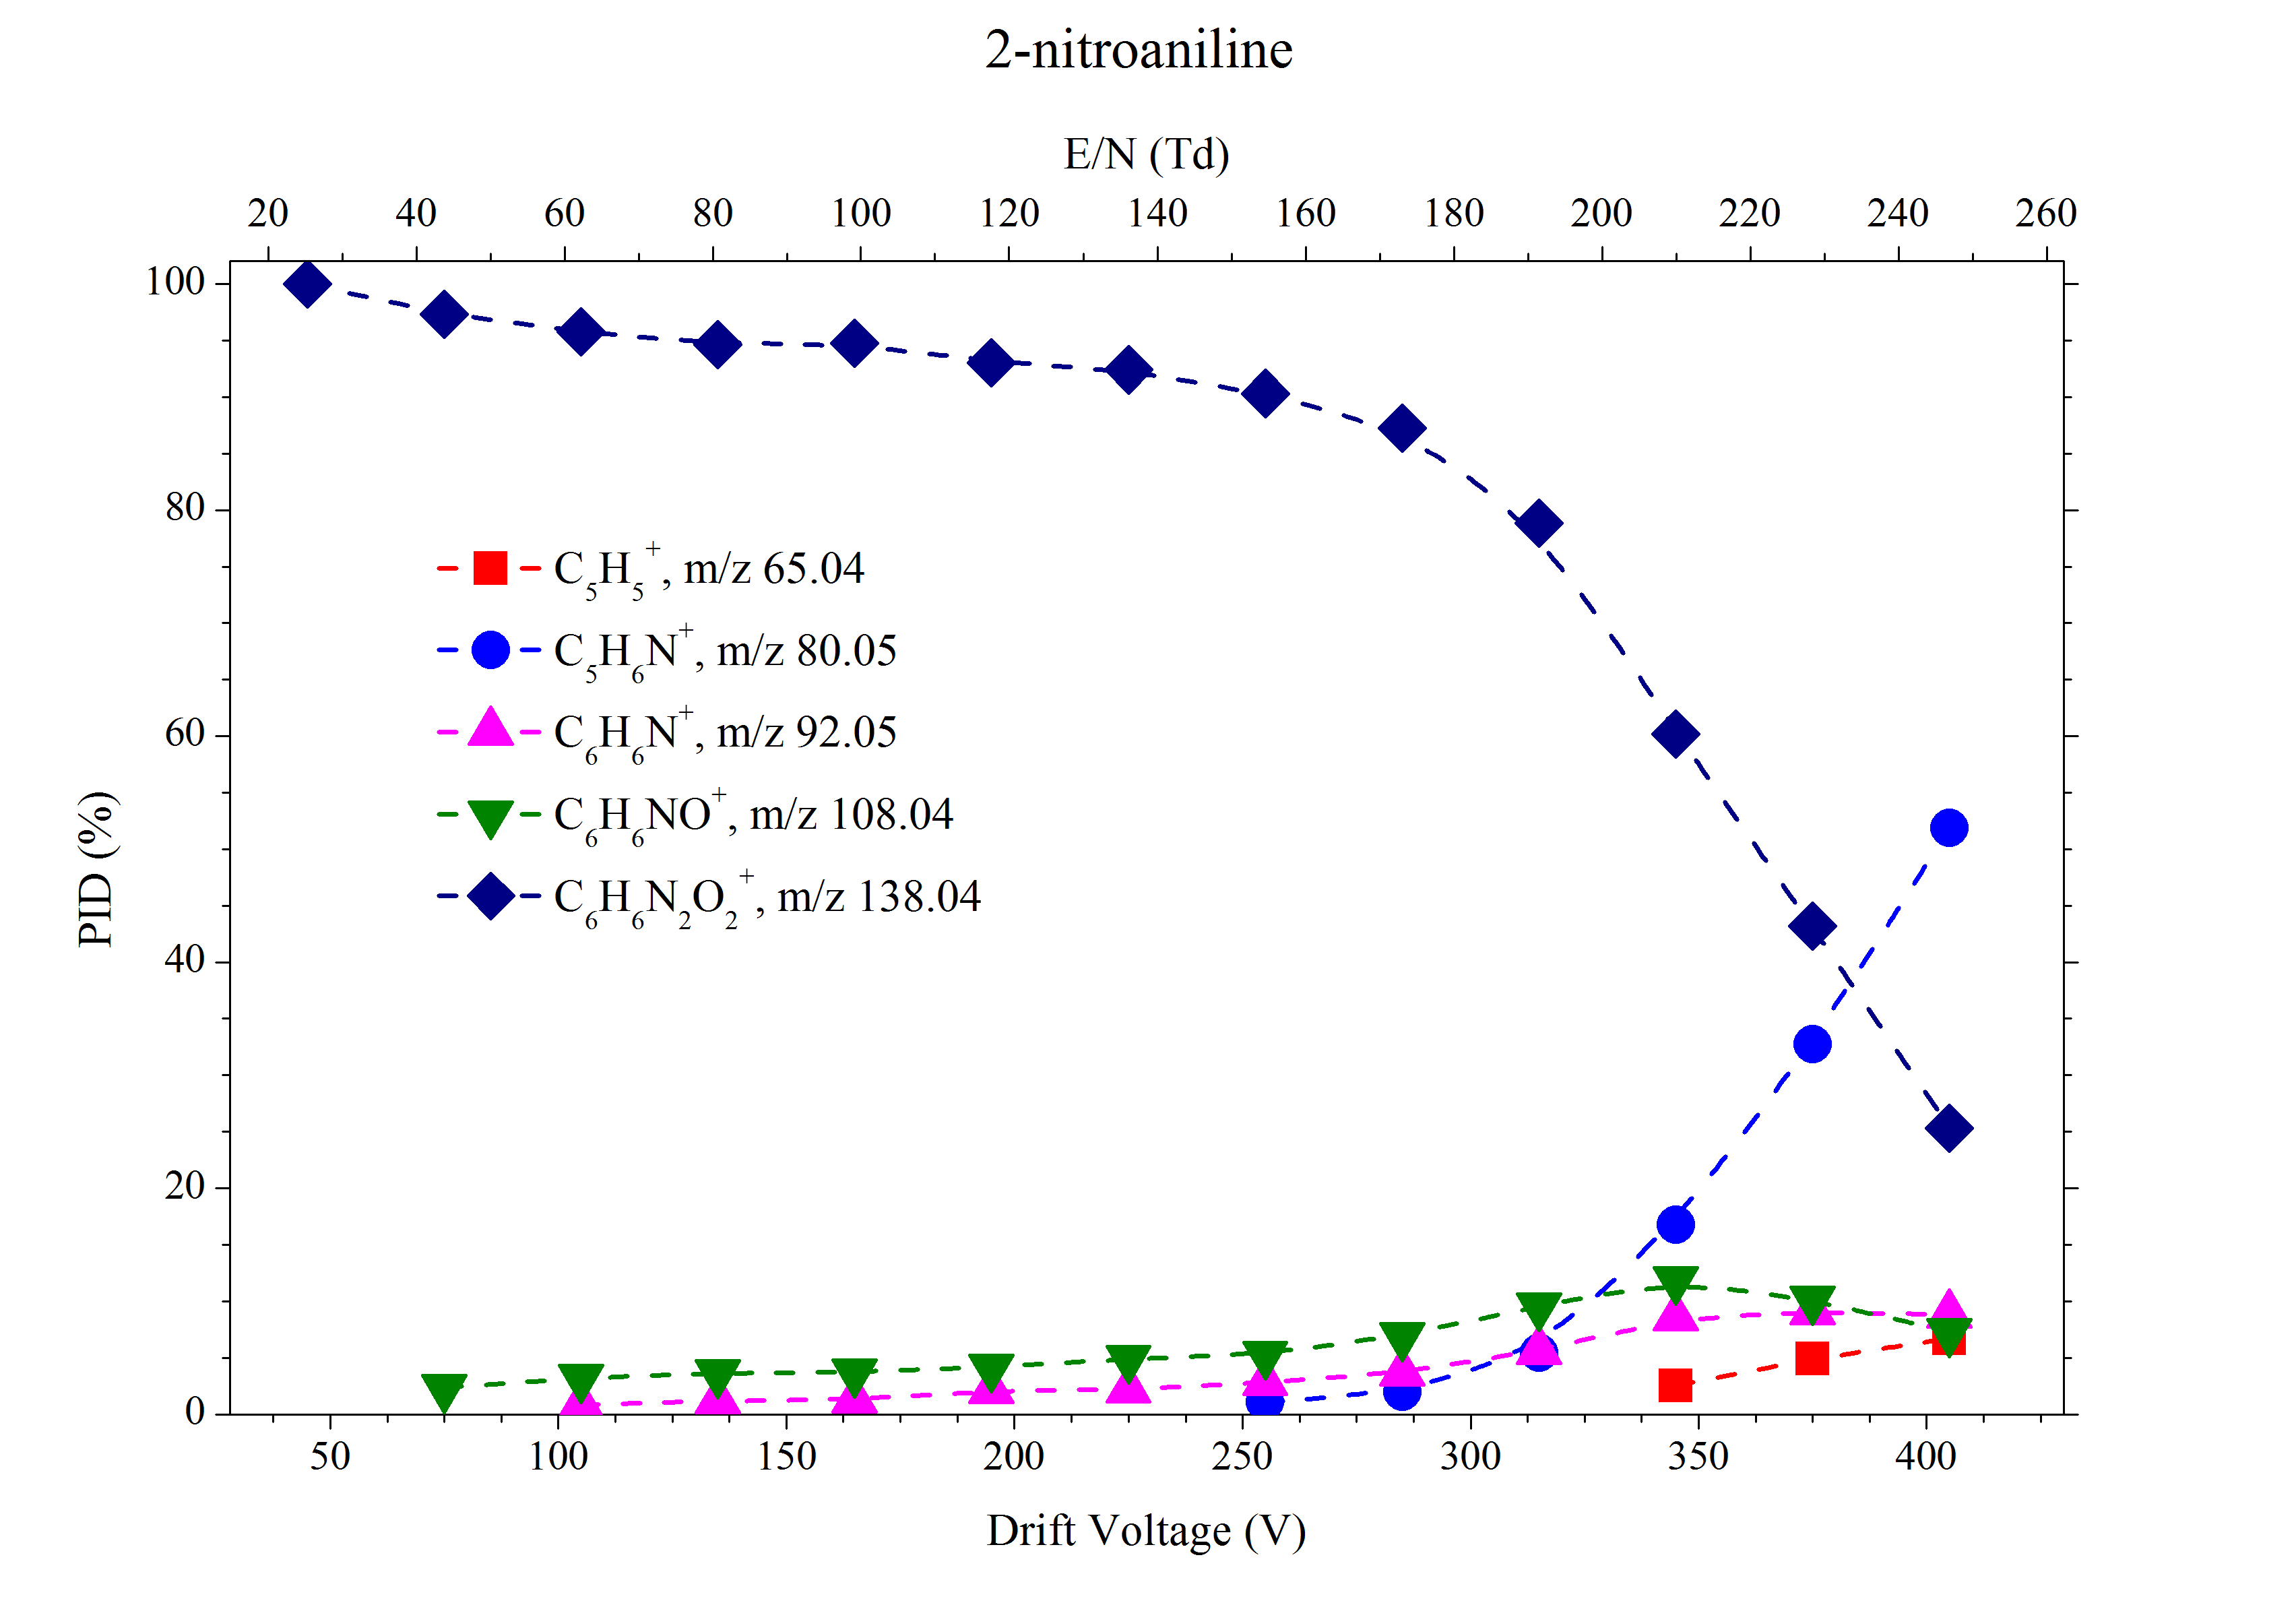
\includegraphics[width=0.6\linewidth]{pics/2-NA-o2_DC.png}}

\sidesubfloat[]{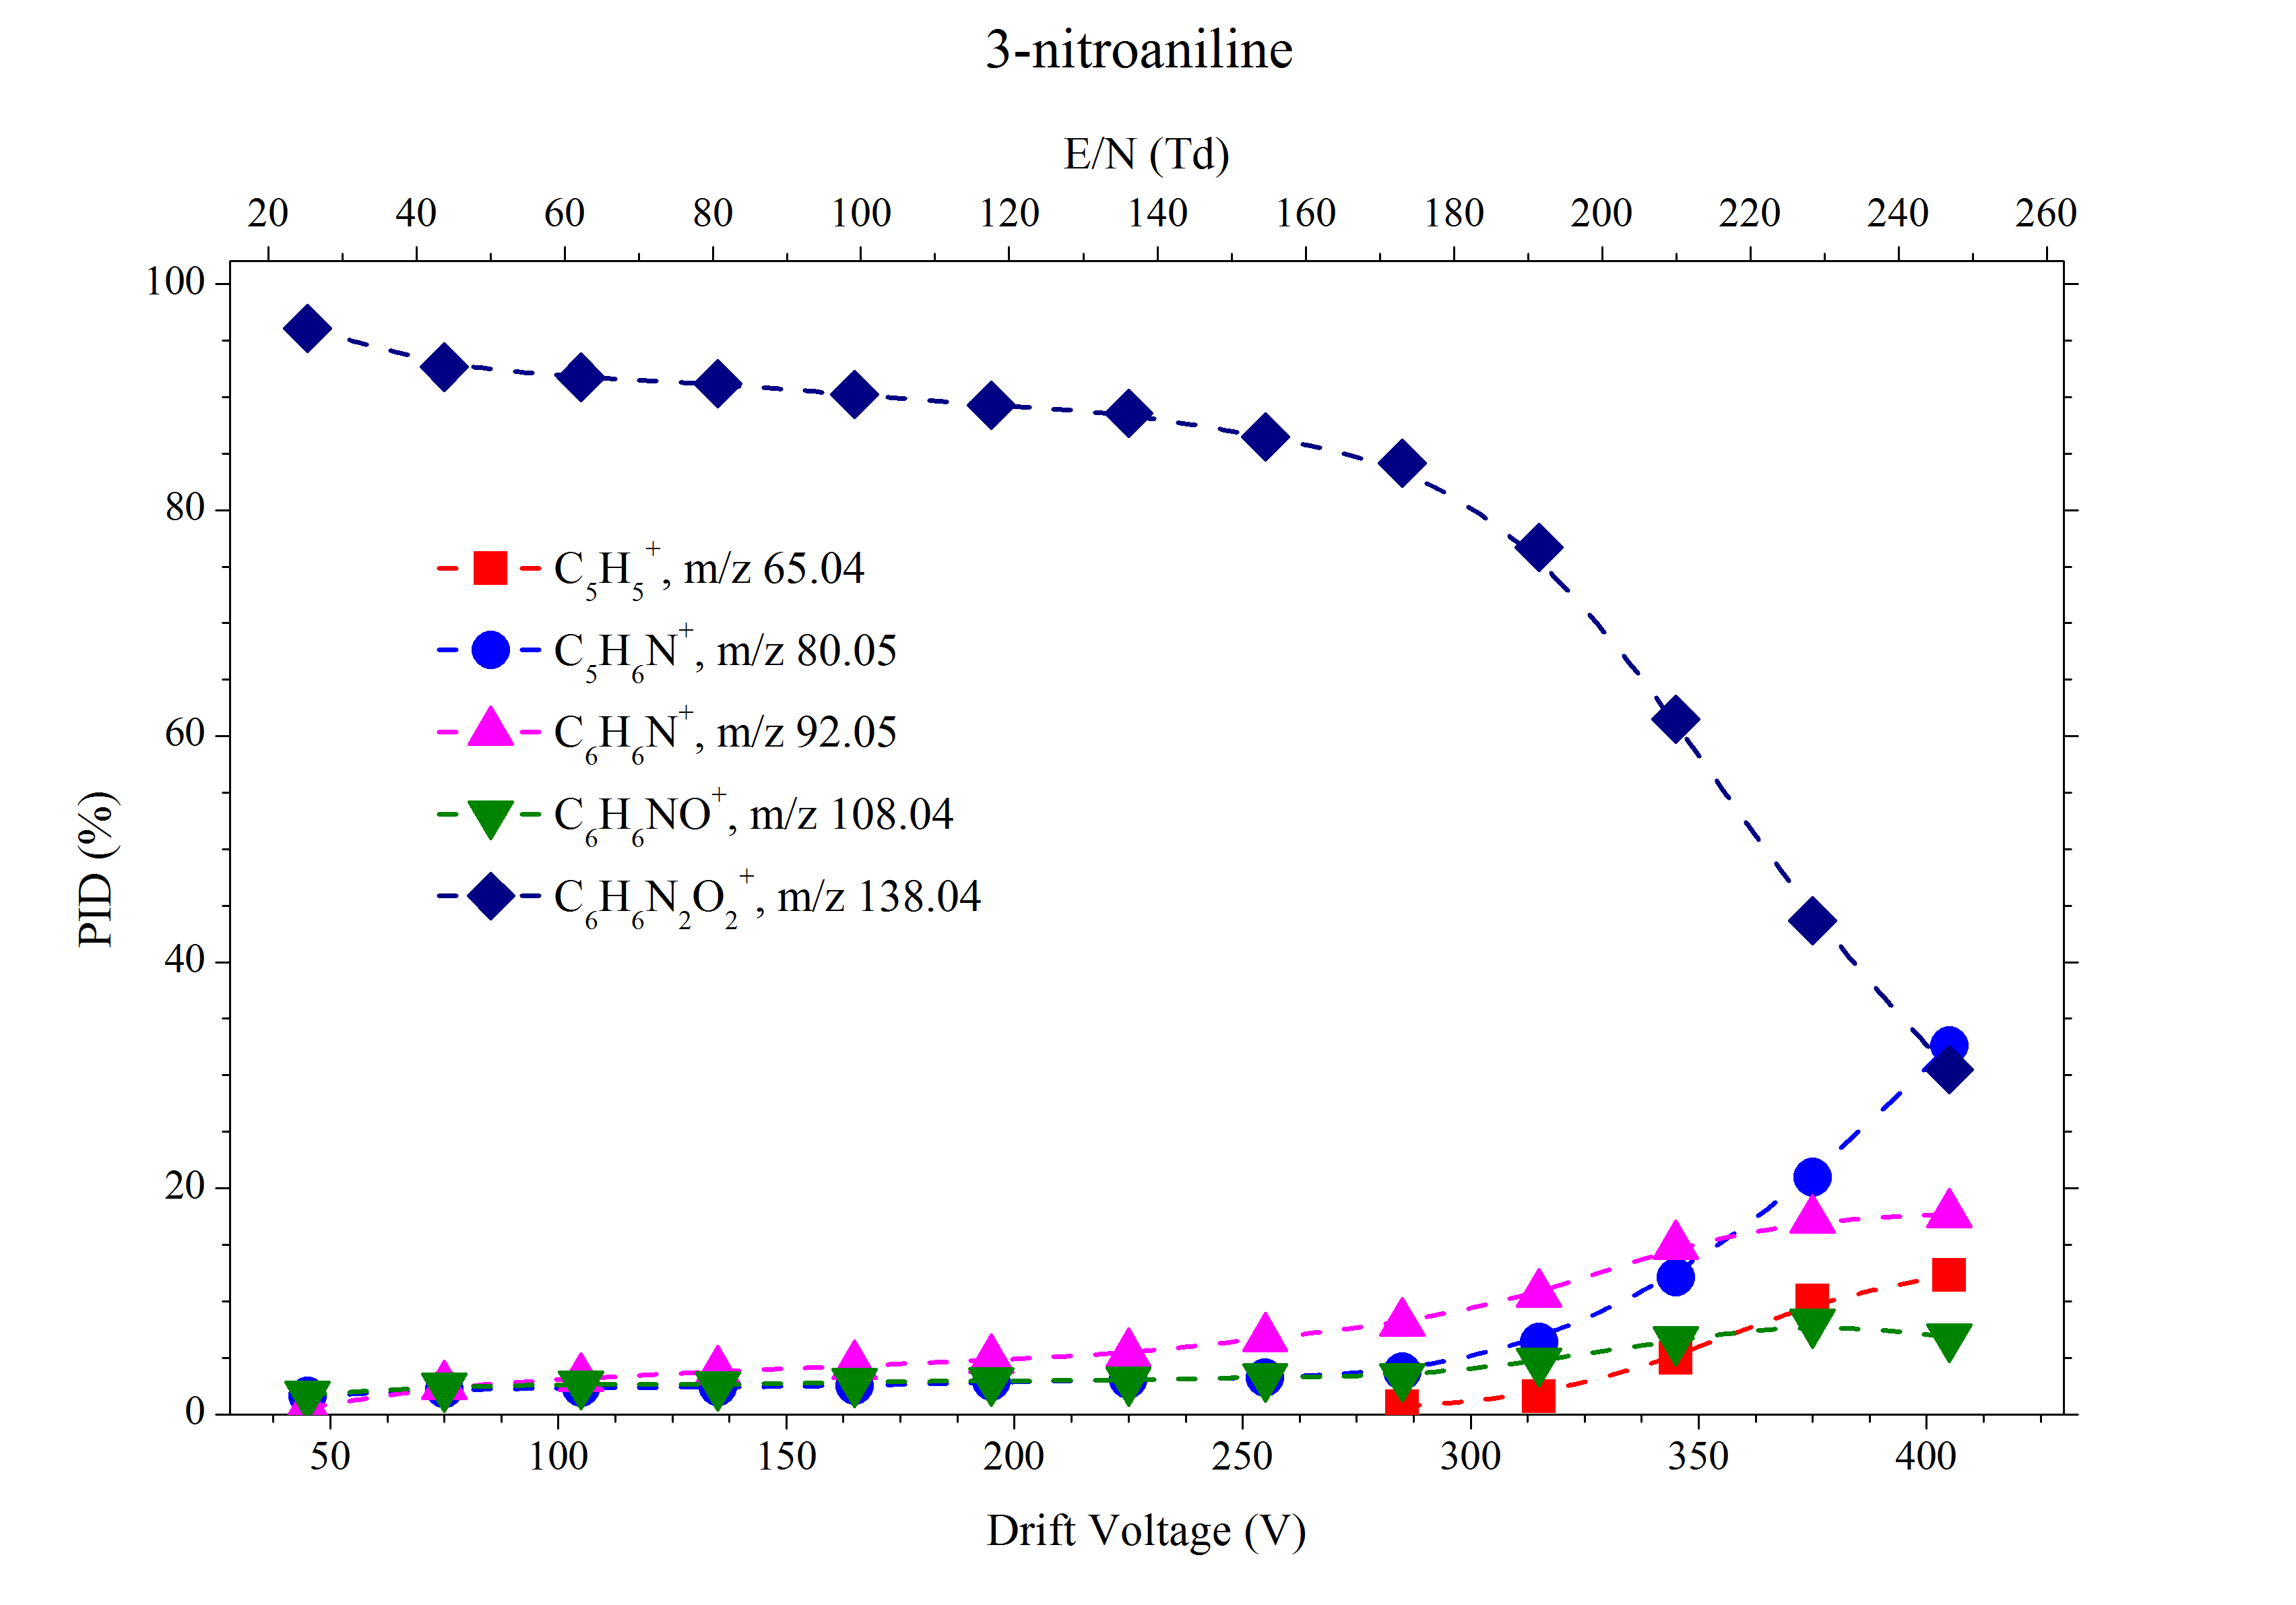
\includegraphics[width=0.6\linewidth]{pics/3-NA-o2_DC.png}}

\sidesubfloat[]{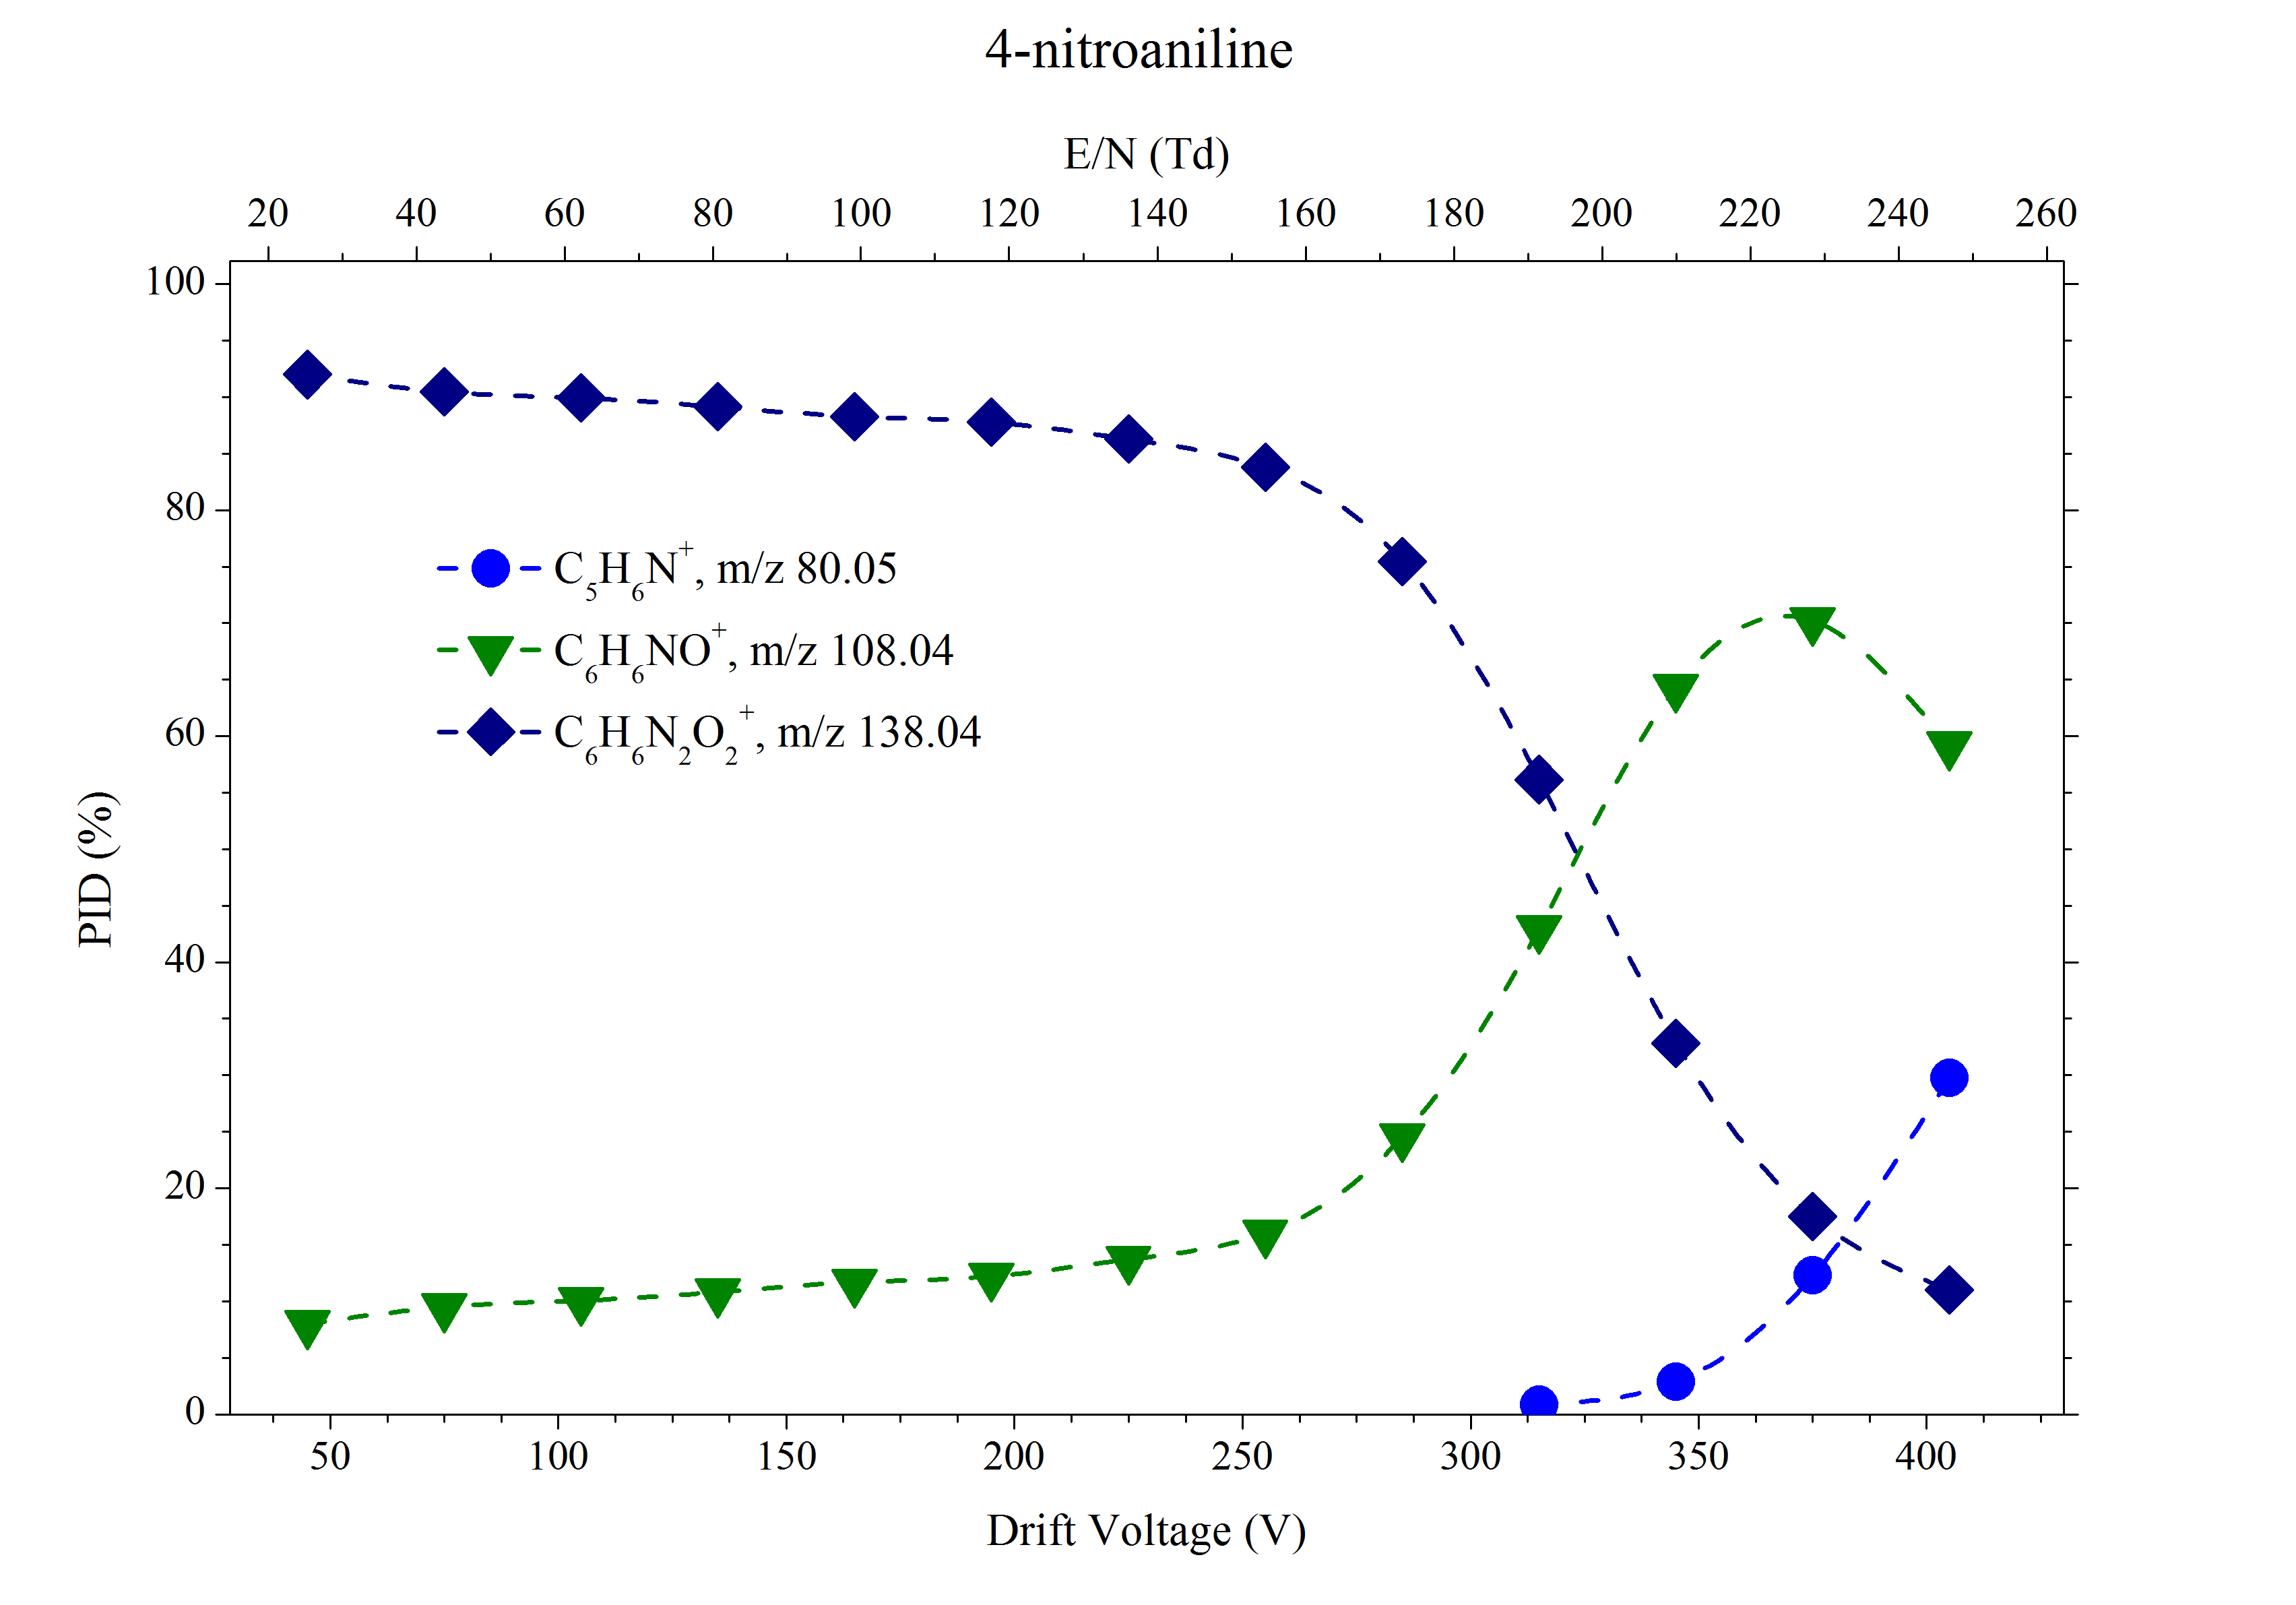
\includegraphics[width=0.6\linewidth]{pics/4-NA-o2_DC.png}}
\caption{PID plots of (a) 2-nitroaniline, (b) 3-nitroaniline and (c) 4-nitroaniline, O2+, DC mode}
\label{fig:na_o2_dc}
\end{figure}




\subsection{Characterisation of the TDU: temperature study}

\subsubsection{HMTD}
Using ------------------- as probe I have done a temperature study of the TDU keeping the rest of the temperatures and pressures constant.

Use HMTD for this (I can't put this in my thesis as it is in a paper already. put reference to the paper)   

\textbf{use the counts per second!!! It is what makes sense}

I measured at different TDU temperatures: 100$^{\circ}$C, 150$^{\circ}$C and 200$^{\circ}$C, while keeping the inlet line and the oven at 150$^{\circ}$C, so the differences come purely from the TDU temperature


\begin{figure}
\scalebox{0.7}{\begin{tikzpicture}\chemfig{N(-[::90,,,,line width=3pt]>[::-30]O-[::-30]O-[::-45]-[::-75]N?[b])(-[::-30,,,,line width=3pt]>[::30]O-[::30]O-[::30]?[b])(-[::-150,,,,line width=3pt]>[::-135]O-[::-45]O-[::-30]?[b])
}\end{tikzpicture}}
\caption{Structure of HMTD.}\label{fig:hmtd}
\end{figure}

\subsubsection{Benzoylecgonine}
Add measurements from 31st October 2018 (latex report)



\section{Conclusions and further remarks}













